

%% ----------------------------------------------------------------
%% Thesis.tex -- MAIN FILE (the one that you compile with LaTeX)
%% ---------------------------------------------------------------- 

% Set up the document
\documentclass[a4paper, 12pt, oneside]{Thesis}  % Use the "Thesis" style, based on the ECS Thesis style by Steve Gunn
\graphicspath{{Figures/}}  % Location of the graphics files (set up for graphics to be in PDF format)
\usepackage[portuguese]{babel}


%mudar margens laterais
\oddsidemargin 32mm
\evensidemargin 32mm


% Include any extra LaTeX packages required
\usepackage[square, numbers, comma, sort&compress]{natbib}  % Use the "Natbib" style for the references in the Bibliography
\usepackage[T1]{fontenc}
\usepackage{verbatim}  % Needed for the "comment" environment to make LaTeX comments
\usepackage{vector}  % Allows "\bvec{}" and "\buvec{}" for "blackboard" style bold vectors in maths
%\usepackage{graphicx}
\usepackage{float}
\usepackage{graphics}
\usepackage{amsmath, amssymb}
\usepackage{eurosym}
\usepackage{tabularx}
\usepackage{fancyhdr}
\usepackage{lastpage}
\usepackage{alltt}
\usepackage{graphicx}
\usepackage{verbatim}
\usepackage{color}
\usepackage{url}
\usepackage{amsmath}
\usepackage{epsf}
\usepackage{float}
\usepackage{multirow}
\usepackage[final]{pdfpages}
\usepackage[nottoc,notbib]{tocbibind}
%\usepackage[notlof]{tocbibind}
\usepackage{thumbpdf}
%\usepackage[latin1]{inputenc}

\usepackage[utf8x]{inputenc}
\usepackage{todonotes}
\usepackage{fancyvrb}
\usepackage{float}
\usepackage{listings}
\renewcommand{\lstlistingname}{Exemplo}% Listing -> Algorithm





\newcommand{\X}{\mathcal{X}}


\hypersetup{urlcolor=blue, colorlinks=true}  % Colours hyperlinks in blue, but this can be distracting if there are many links.


%% ----------------------------------------------------------------
\begin{document}

\frontmatter	  % Begin Roman style (i, ii, iii, iv...) page numbering

%COVER PAGE%
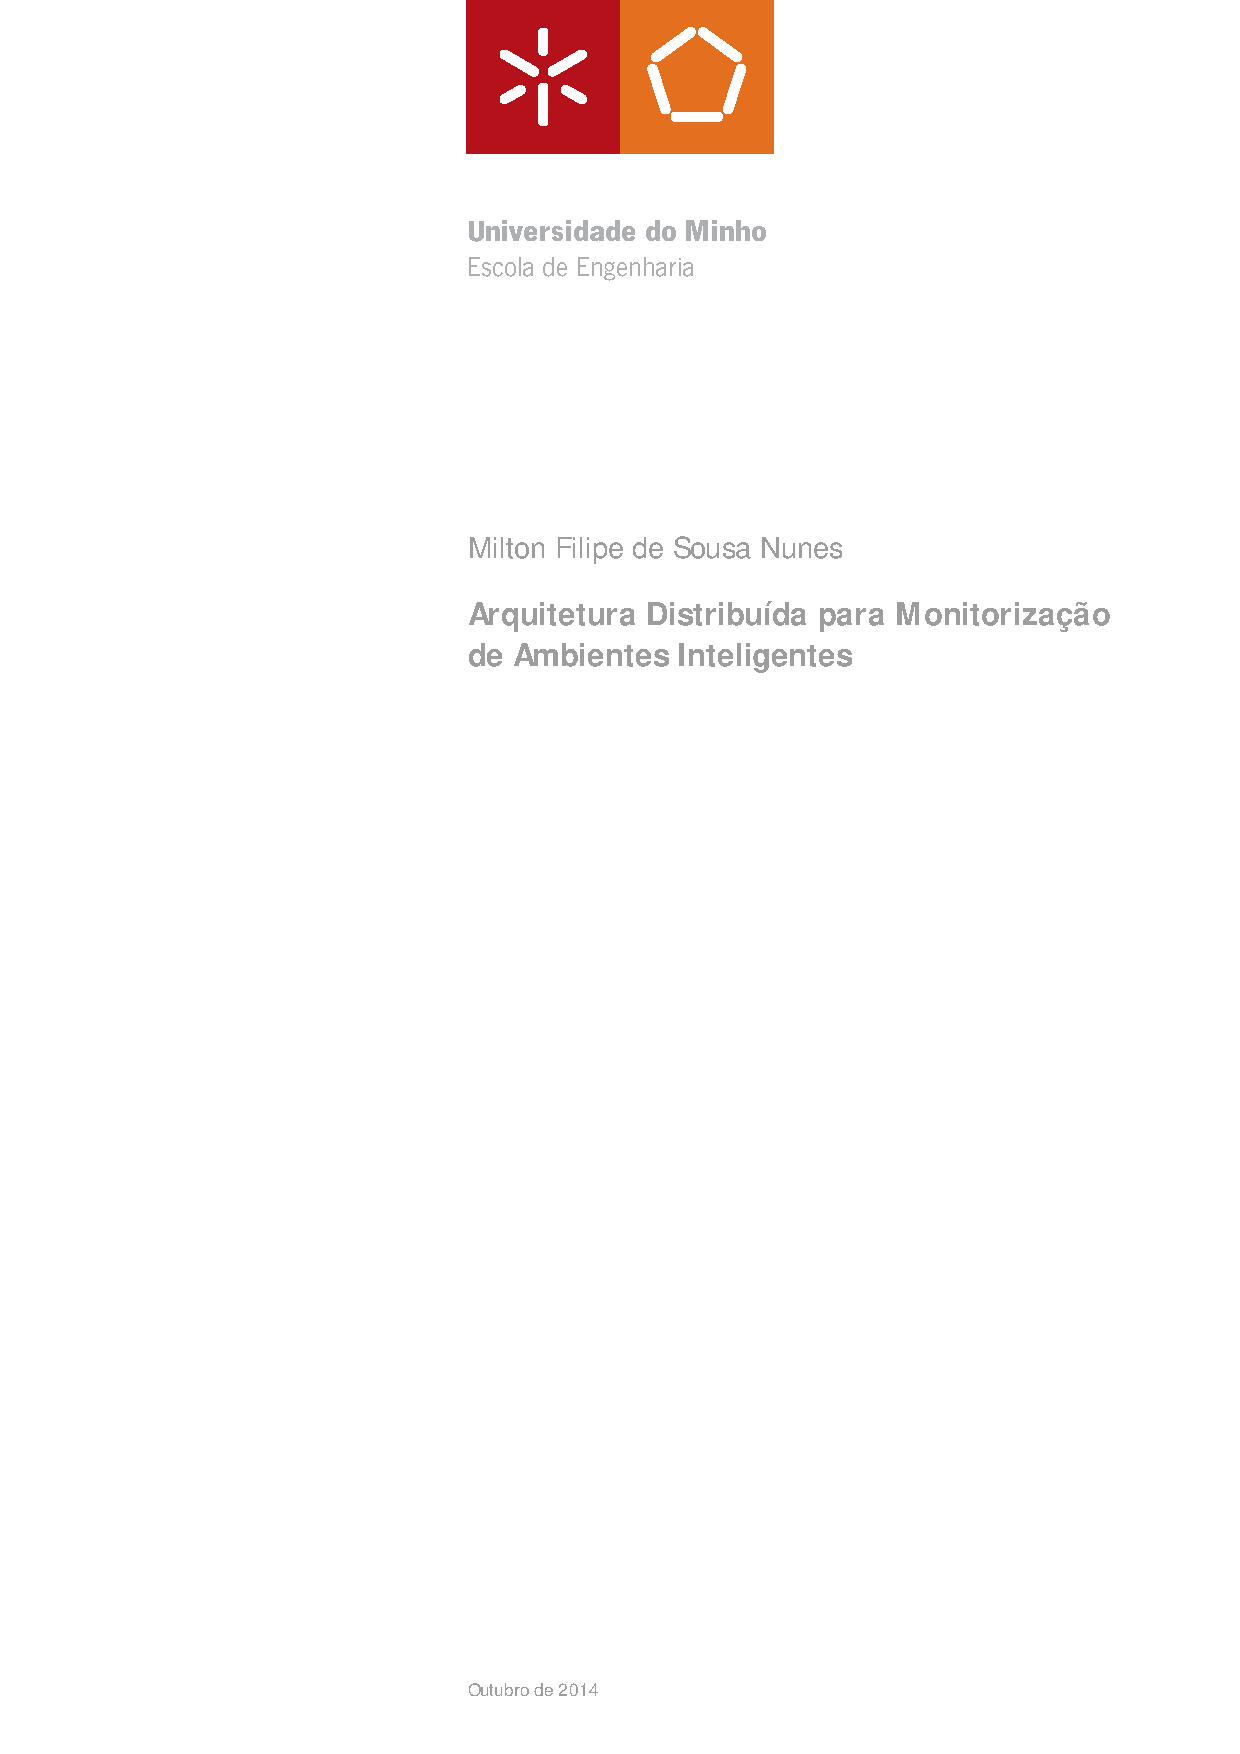
\includepdf[pages=1,scale=1,offset=2.5cm -2.5cm]{capatese1.pdf}
\includepdf[pages=2,scale=1,offset=2.5cm -2.5cm]{capatese1.pdf}
%% ----------------------------------------------------------------

\setstretch{1.5}  % It is better to have smaller font and larger line spacing than the other way round
\onehalfspacing
% Define the page headers using the FancyHdr package and set up for one-sided printing
\fancyhead{}  % Clears all page headers and footers
\rhead{\thepage}  % Sets the right side header to show the page number
\lhead{}  % Clears the left side page header

\pagestyle{fancy}  % Finally, use the "fancy" page style to implement the FancyHdr headers

%% ----------------------------------------------------------------
% Declaration Page required for the Thesis, your institution may give you a different text to place here

\clearpage  % Declaration ended, now start a new page

%% ----------------------------------------------------------------
% The "Funny Quote Page"
%\pagestyle{empty}  % No headers or footers for the following pages
%
%\null\vfill
% Now comes the "Funny Quote", written in italics
%\textit{``If we could unfold the future, the present would be our greatest care.''}
%
%\begin{flushright}
%Edward Counsel, Maxims
%\end{flushright}
%
%\vfill\vfill\vfill\vfill\vfill\vfill\null
%\clearpage  % Funny Quote page ended, start a new page
%% ----------------------------------------------------------------

%----------------Agradecimentos----------------


%\addtotoc{Agradecimentos}
\chapter*{Agradecimentos}

A conclusão deste trabalho não seria possível sem a ajuda e apoio de um conjunto de pessoas. Deixo-lhes aqui o meu sincero agradecimento:


Aos meus orientadores Professor Paulo Novais e Davide Carneiro pelo constante acompanhamento, apoio, sugestões e incentivo dado durante todo o trabalho.

Ao meu amigo e colega de trabalho do ISLab André Pimenta por todo o apoio, pelas suas ideias, e pela sua constante disponibilidade.

A todos os meus colegas de curso e amigos que comigo iniciaram o seu percurso académico e estiveram sempre ao meu lado.

E ainda um agradecimento muito especial aos meus pais Milton Nunes e Adélia Sousa, e à minha irmã Magda Nunes, por todo incentivo e força que me deram durante todo este percurso.

\newpage
\thispagestyle{empty}
\mbox{}

\include{asas}



% !TEX encoding = IsoLatin
%\thispagestyle{empty}
\begin{center}
{\large \textit{Resumo} }
\end{center}
%\newenvironment{resumo}
%{\thispagestyle{empty} \vspace*{\stretch{1}}\begin{flushleft} \em}{\end{flushleft} \vspace*{\stretch{3}}}


\vspace{0.5cm}
\quad Existe atualmente uma grande facilidade no acesso à informação e um interesse generalizado em utilizar essa informação para aumentar a comodidade e bem estar das pessoas. O conhecimento é reconhecidamente uma arma poderosa que tende ser explorada até ao limite. Desta forma importa encontrar todas as fontes de informação que possam ser úteis para alcançar esse objetivo global. Neste sentido o potencial da informação ambiente que rodeia um ser humano é enorme e a falta de aproveitamento verificada sobre esse conhecimento é uma falha que deve ser colmatada. Existem nesta perspetiva várias formas de aplicação deste conhecimento, entre as quais a possibilidade de proporcionar melhores condições de vida e de bem estar. Pretende-se assim com este trabalho desenvolver uma arquitetura composta por sensores colocados de forma distribuída capaz de monitorizar ambientes inteligentes com base em diversos fatores. Nesta arquitetura a função de cada sensor pode ser vista como um serviço prestado aos seus utilizadores, através dos quais são recolhidos diferentes tipos de informação. Este trabalho, através dos vários indicadores recolhidos, oferece aos seus utilizadores o acesso a diversas informações sobre o seu comportamento e reações durante o período de monitorização.

\vspace{3cm}

\textbf{Palavras-chave:} Arquitetura, Serviços, Ambientes Inteligentes, Monitorização, Sensores




\newpage
\thispagestyle{empty}
\mbox{}
%----------------Abstract----------------

%\addtotoc{Abstract}  % Add the "Abstract" page entry to the Contents
% !TEX encoding = IsoLatin
\begin{center}
{\large \textit{Abstract} }
\end{center}
%\newenvironment{resumo_ingles}
%{\thispagestyle{empty} \vspace*{\stretch{1}}\begin{flushleft} \em}{\end{flushleft} \vspace*{\stretch{3}}}






%{\centering \large
%{\large\bf \textbf{Abstract} } }

\vspace{0.5cm}
\quad Nowadays there is a great ease in accessing information and widespread interest in using  this information to increase the comfort and welfare of people. Knowledge is recognized as a powerful weapon that tends to be exploited to the limit. Thus matter find all the sources of information that may be helpful to achieve this global goal. In this sense, the potential of environment information surrounding a human being is huge and the lack of exploitation that occurs on that knowledge is a fault that should be corrected. Given this perspective there are several ways of applying this knowledge, including the ability to provide better living conditions and welfare. The aim of this work is to develop an architecture composed by sensors placed in a distributed way, capable of monitoring an ambient intelligence based on several factors. In this architecture the function of each sensor can be viewed as a service to its users, being collected through them different types of information. This work, through the several indicators collected, offers its users access to diverse information about their behaviour and reactions during  the monitoring period.
\vspace{3cm}

\textbf{Key Words:} Architecture, Services, Ambient Intelligence, Monitoring, Sensors.
\newpage
\thispagestyle{empty}
\mbox{}


%% ----------------------------------------------------------------

\pagestyle{fancy}  %The page style headers have been "empty" all this time, now use the "fancy" headers as defined before to bring them back

%% ----------------------------------------------------------------
\lhead{\emph{Conteúdo}}  % Set the left side page header to "Contents"
\tableofcontents  % Write out the Table of Contents

%% ----------------------------------------------------------------
%\lhead{\emph{Lista de figuras}}  % Set the left side page header to "List if Figures"
\renewcommand\listfigurename{Lista de Figuras}
\listoffigures  % Write out the List of Figures

%% ----------------------------------------------------------------
%\lhead{\emph{Lista de figuras}}  % Set the left side page header to "List of Tables"
\renewcommand\listtablename{Lista de Tabelas}
\listoftables  % Write out the List of Tables
\newpage

\newpage
\thispagestyle{empty}
\mbox{}
%% ----------------------------------------------------------------
\setstretch{1.5}  % Set the line spacing to 1.5, this makes the following tables easier to read
\clearpage  % Start a new page
\lhead{\emph{Abreviaturas}}
\addtotoc{Abreviaturas}

{\centering \LARGE
{\LARGE\bf \textbf{Abreviaturas} } }\\\\


\begin{table}[!h]
\begin{tabular}{ll} 
	\textbf{CAMCoF}	& \textbf{C}ontext \textbf{M}ultimodal  \textbf{C}omunication \textbf{F}ramework	 \\ \\
	\textbf{AmI}	& \textbf{Am}bient \textbf{I}ntelligence	 \\ \\
	\textbf{REST}	& \textbf{Re}presentational \textbf{S}tate \textbf{T}ransfer	 \\ \\
	\textbf{SOAP}	& \textbf{S}imple \textbf{O}bject  \textbf{A}ccess \textbf{P}rotocol	 \\ \\
	\textbf{XML}	& e\textbf{X}tensible \textbf{M}arkup  \textbf{L}anguage	 \\ \\
	\textbf{JSON}	& \textbf{J}ava\textbf{S}cript  \textbf{O}bject \textbf{N}otation	 \\ \\
	\textbf{HTTP}	& \textbf{H}yper\textbf{T}ext  \textbf{T}ransfer \textbf{P}rotocol	 \\ \\
	\textbf{TCP}	& \textbf{T}ransmission \textbf{C}ontrol  \textbf{P}rotocol	 \\ \\
	\textbf{IP}	& \textbf{I}nternet \textbf{P}rotocol	 \\ \\
	\textbf{URL}	& \textbf{U}niform \textbf{R}esource  \textbf{L}ocator	 \\ \\
	\textbf{API}	& \textbf{A}pplication \textbf{P}rogramming  \textbf{I}nterface  \\ \\
	\textbf{OSGi}	& \textbf{O}pen \textbf{S}ervice  \textbf{G}ateway \textbf{i}nitiative	 \\ \\
	\textbf{XSLT}	& e\textbf{X}tensible \textbf{S}tylesheet  \textbf{L}anguage \textbf{T}ransformations	 \\ \\
	\textbf{BPMN}	& \textbf{B}usiness \textbf{P}rocess  \textbf{M}odel and \textbf{N}otation	 \\ \\
	\textbf{jBPM}	& \textbf{j}ava  \textbf{B}usiness \textbf{P}rocess \textbf{M}anagement	
 \\ \\
	\textbf{URL}	& \textbf{U}niform \textbf{R}esource  \textbf{L}ocator  \\ \\
	\textbf{POM}	& \textbf{P}roject \textbf{O}bject  \textbf{M}odel  \\ \\
	\textbf{SQL}	& \textbf{S}tructured \textbf{Q}uery  \textbf{L}anguage  \\ \\
	\textbf{JSF}	& \textbf{J}ava \textbf{S}erver  \textbf{F}aces  \\ \\
	\textbf{MVC}	& \textbf{M}odel \textbf{V}iew  \textbf{C}ontroller  \\ \\			      	\textbf{ISLab}	& \textbf{I}ntelligent \textbf{S}ystems  \textbf{Lab}  \\ \\
\end{tabular}
\end{table}
\newpage
\thispagestyle{empty}
\mbox{}


%% ----------------------------------------------------------------

% End of the pre-able, contents and lists of things
% Begin the Dedication page

\setstretch{1.3}  % Return the line spacing back to 1.3

\pagestyle{empty}  % Page style needs to be empty for this page


\addtocontents{toc}{\vspace{2em}}  % Add a gap in the Contents, for aesthetics


%% ----------------------------------------------------------------
\mainmatter	  % Begin normal, numeric (1,2,3...) page numbering
\lhead[\rm\thepage]{\fancyplain{}{\sl{\rightmark}}}
\pagestyle{fancy}  % Return the page headers back to the "fancy" style

% Include the chapters of the thesis, as separate files
% Just uncomment the lines as you write the chapters

\chapter{Introdução}

O ambiente que rodeia um indivíduo encontra-se repleto de informação que é normalmente ignorada mas que pode ser utilizada de diversas formas em seu proveito. É possível utilizar essa informação ambiente para proporcionar maior conforto, promover o seu bem estar e até contribuir para a sua saúde física e mental. Através da utilização de sensores que monitorizem comportamentos e ações de um ser humano é possível efetuar recolhas de dados, que depois de processados poderão revelar indicadores da ocorrência de fatores como por exemplo a fadiga ou stress. A partir deste levantamento de informação é possível retirar conclusões que permitam promover a qualidade de vida de um indivíduo, contribuir para o seu bem estar e para a sua saúde. 

Um exemplo prático que retrata este tipo de situações é por exemplo a monitorização de uma estrada em que se registe um elevado número de acidentes. Através da sua monitorização poder-se-ia analisar as suas condições, a condução dos seus utilizadores, as alterações na condução perante mudanças climatéricas, entre outras situações. Com base nos resultados desta monitorização seria então possível retirar conclusões que permitissem evitar a ocorrência de tantos acidentes.


\section{Motivação}
O registo da informação ambiente que é por diversas vezes desaproveitada, pode ser feito através do recurso a dispositivos eletrónicos como os sensores. Estes dispositivos, de fácil acesso e utilizado nos mais diversos contextos, têm a capacidade de identificar e responder a estímulos de forma a convertê-los em sinais que podem assim ser registados e armazenados\cite{akyildiz2002wireless}. 

Existe atualmente no mercado um conjunto bastante diversificado de sensores, capazes de identificar vários tipos de indicadores, como os sensores de luz, movimento ou temperatura. Uma das grandes vantagens deste tipo de dispositivos é a diversidade de indicadores que estes permitem identificar e registar. Contudo este potencial proporcionado pela diversidade de sensores não é ainda suficientemente aproveitado, dado que a utilização destes dispositivos é feito na maior parte das vezes de forma isolada, descurando-se assim a possibilidade de estabelecer uma relação entre os vários indicadores levantados e construir uma visão global \cite{salber1999designing} sobre a informação presente num ambiente que se pretende inteligente \cite{ducatel2001scenarios, ducatel2003ambient}.

Assim, este trabalho é motivado pela criação de uma arquitetura que possa colmatar esta questão. Dessa forma pretende-se integrar numa arquitetura sensores de diversos tipos, de forma distribuída, capaz de recolher vários tipos de indicadores e armazenar essa informação. Esta arquitetura vem resolver o problema da dispersão dos dados e permitir a monitorização de um ambiente inteligente, disponibilizando por fim um vasto leque de informações recolhidas através dos dispositivos integrados.

Este trabalho está diretamente ligado a áreas como por exemplo a saúde, psicologia e militar \cite{akyildiz2002wireless, aarts2006into}. Estas áreas têm grande interesse em sistemas que através do uso de dispositivos como sensores, permitam a monitorização e recolha de dados ambiente, dando assim suporte ao desenvolvimento de estudos relacionadas com estados como o stress e fadiga ou à disponibilização de determinado serviço. Posto isto, estas são áreas que terão obviamente o seu foco direcionado para uma solução como a arquitetura descrita.


\section{Âmbito da Dissertação}
Uma pessoa quando se encontra tanto no seu período de trabalho como fora dele, está sujeito a diversos fatores que provocam reações físicas e psicológicas que por vezes este nem sequer se apercebe. Contudo estas reações têm implicações no seu rendimento, no seu comportamento e até porventura no seu futuro. Todas estas reações são, na maior parte das vezes, impercetíveis à \textit{vista desarmada}, contudo podem ser identificadas e registadas com o recurso a dispositivos como os sensores. Através da utilização deste tipo de tecnologias é possível recolher um conjunto alargado de indicadores, que podem assim ser analisados e retirar conclusões sobre o comportamento e consequente bem estar de um indivíduo envolvido num ambiente inteligente, com o intuito de proporcionar-lhe cada vez melhores condições.

Posto isto, pretende-se com este trabalho desenvolver uma arquitetura composta por sensores colocados de forma distribuída que recolham dados de diversas fontes de informação, monitorizando desta forma indivíduos num ambiente inteligente. A informação recolhida pretende-se que seja armazenada numa unidade central de modo a que seja possível consultar e relacionar facilmente os diversos tipos de dados. Assim pretende-se, para além de monitorizar um ambiente inteligente, automatizar a recolha dos dados provenientes dos diversos serviços alocados de forma distribuída e facilitar a sua gestão.


\section{Principais Desafios}

A recolha de informação ambiente que circunda um indivíduo é uma tarefa que requer alguma sensibilidade. Esta deve ser efetuada com bastante cuidado pois os métodos utilizados nesta tarefa devem evitar interferir com o comportamento natural do indivíduo, para garantir a fiabilidade da informação recolhida. Desta forma, deve ser efetuada uma monitorização constante sobre os seus utilizadores de modo a que seja possível recolher um número considerável de dados, que abranjam diferentes situações e momentos, com diferentes características e em diversos âmbitos. Esta diversidade é extremamente importante pois permitirá verificar oscilações, comparar diferentes contextos e verificar diferentes comportamentos e reações.

Para além dos contextos e situações de monitorização, é fundamental que a amostra proveniente  dos utilizadores consiga abranger vários tipos de indicadores. Existem vários tipos de informação que pode ser recolhida, dando origem a diferentes indicadores a ter em conta sobre cada utilizador. Esta diversidade de informação é muito importante pois determina a fiabilidade do conjunto de dados levantados e acrescenta solidez e precisão à monitorização efetuada sobre cada indivíduo.

Tendo como base a existência de diversos contextos e tipos de informação, provenientes de diferentes sensores, é essencial também automatizar toda a gestão de serviços que farão parte da arquitetura. Estes serviços que se encontram associados a diferentes tipos de sensores, deverão ter a capacidade de efetuar periodicamente comunicações com a uma unidade central com o intuito de automaticamente gerar fluxos de informação para que esta esteja facilmente acessível. A funcionalidade da aplicação dependerá diretamente da acessibilidade aos dados levantados, dado que o principal propósito da recolha de informação ambiente é que esta esteja disponível para que possa ser utilizada em prol dos seus utilizadores.

A utilização de vários sensores para recolha de informação e a importância da sua comunicação implica que a arquitetura garanta a interoperabilidade dos componentes nela integrados. Os diversos dispositivos que constituem a arquitetura devem conseguir comunicar de modo transparente, permitindo a assim uma troca efetiva e eficiente de informação. Esta característica assegura a cooperação dos diversos tipos de sensores que compõem a arquitetura e permite adicionar novos dispositivos de forma automática.

\section{Objetivos}

O objetivo deste trabalho é desenvolver uma arquitetura composta por vários tipos de sensores distribuídos para a monitorização dos seus utilizadores e consequente recolha de informação ambiente. Para isso é necessário desenvolver métodos que permitam a cooperação de diferentes dispositivos capazes de recolher informação e tratar do seu envio para uma unidade central onde esta será armazenada. Com o intuito de construir uma arquitetura o mais abrangente possível, esta será composta por fontes de informação diversificadas podendo ter como origem dispositivos como computadores, dispositivos móveis e até unidades de biofeedback.

A criação de uma unidade central onde a informação é armazenada deve-se ao facto de estruturalmente ser mais fácil processar e aceder os dados recolhidos. Desta forma os dados de cada utilizador tornam-se facilmente acessíveis, podendo ser analisados, comparados os diversos tipos de dados, verificadas as oscilações ocorridas e ainda constatar a evolução ao longo de todo o período de monitorização.

Posto isto, enumera-se de seguida os principais objetivos a alcançar com este trabalho:
\begin{itemize}
  \item Criar arquitetura composta por sensores distribuídos através da framework SwitchYard baseada na linguagem de programação Java.
  \item Implementar métodos de comunicação que permitam a cooperação e a transmissão de dados entre os componentes da arquitetura.
  \item Assegurar a interoperabilidade dos diferentes componentes integrados na arquitetura.
  \item Agregar toda a informação proveniente dos vários serviços numa unidade central.
  \item Identificar a existência de novos serviços e integrá-los automaticamente na arquitetura.
  \item Fazer a gestão dos dados armazenados na unidade central.
  \item Desenvolver uma página web na qual os utilizadores consigam aceder aos seus dados.
  \end{itemize}


\section{CAMCoF}
Este trabalho está integrado num projeto de maior dimensão denominado Context-aware Multimodal Communication Framework\footnote{http://islab.di.uminho.pt/camcof/index.php}. Este tem como objetivo desenvolver uma framework para modelação do contexto de um utilizador com base na ocorrência de stress. Sendo este estado estimado tendo em conta a análise do comportamento de indivíduos e os seus padrões de interação.

Através da utilização da informação recolhida, o CAMCoF pretende ainda desenvolver um ambiente virtual que permita que os seus utilizadores tenham acesso a processos de comunicação semelhantes à comunicação cara-a-cara. Pretende-se também que a framework seja não-intrusiva e não-invasiva, características que permitirão que a monitorização efetuada seja o mais frequente e precisa possível.

\section{Estrutura do Documento}

Estruturalmente este documento encontra-se dividido em sete capítulos abordando cada um dos seguintes temas: Introdução, Ambientes Inteligentes, Arquitetura Orientada a Serviços, Arquitetura Desenvolvida, Validação da Arquitetura, Interface Web e Conclusões e Trabalho Realizado. 

O capítulo seguinte refere-se aos Ambientes Inteligentes no qual é abordado em que consistem, a importância da Informação Ambiente, a sua função como um serviço apresentado aos seus utilizadores, em que consiste a Monitorização e ainda alguns exemplos de Sistemas de Monitorização existentes e quais as suas características.

O capítulo 3 define em que consiste uma Arquitetura Orientada a Serviços, as características da arquitetura definida, a importância da utilização de sensores na arquitetura, a forma como a informação é armazenada, as tecnologias utilizadas e ainda algumas decisões tomadas no que ao contexto tecnológico diz respeito, bem como o fundamento dessas decisões.

O quarto capítulo aborda toda as questões relacionadas com a implementação da arquitetura, nomeadamente todas as decisões tomadas, métodos utilizados na implementação de comunicação, armazenamento de dados e assuntos relacionados.

O capítulo 5 apresenta a experiência efetuada para validar a funcionalidade, utilidade e características da aplicação desenvolvida. São apresentados todos os pressupostos definidos para a demonstração e ainda todos os resultados obtidos através desta experiência.

O sexto capítulo apresenta a interface Web desenvolvida para que os utilizadores da plataforma consigam aceder aos seus dados. Neste capítulo é apresentado o padrão de desenvolvimento utilizado, os tipos de acesso de utilizadores implementados, os resultados de monitorização dos utilizadores e ainda as funcionalidades de administração existentes.

No último capítulo, Conclusões e Trabalho Realizado, são apresentadas todas as conclusões e síntese do trabalho realizado nesta dissertação e ainda alguns pontos para trabalho futuro que aumentariam a qualidade da solução apresentada.

 % Introdução

\chapter{Ambientes Inteligentes}

\section{O que são?}

Um Ambiente Inteligente (AmI) \cite{ducatel2001scenarios, ducatel2003ambient} consiste na utilização da informação existente no ambiente e que rodeia um ser humano de forma a facilitar a realização de tarefas ou disponibilizando serviços com o intuito promover a sua comodidade e bem estar. Este conceito relativamente recente é visto como uma área ainda em desenvolvimento mas à qual se vaticina um grande impacto no futuro, suscitando elevado interesse em diversas áreas da indústria e saúde, por exemplo \cite{aarts2006into}.

Esta área baseia-se num novo conceito de processamento e utilização de informação ambiente no qual a utilização de vários dispositivos industriais, de investigação científica, elétricos e ligados à computação são uma realidade e apenas conjuntamente é possível a construção de Ambientes Inteligentes. Este suporte proporcionado por aparelhos tecnológicos de diversos tipos é fundamental para tarefas como a identificação, recolha de dados e monitorização da ação humana e do ambiente \cite{ducatel2001scenarios}. Desta forma, os AmI usufruem do desenvolvimento tecnológico corrente para promover a integração de vários dispositivos num ambiente e poder retirar através destes partido da informação ambiente abundante.

Um foco fundamental em Ambientes Inteligentes é a interação com o ser humano \cite{aarts2006into}. O sucesso de um AmI depende muitas vezes da capacidade de interação que um ser humano consegue ter com o sistema, existindo para isso a necessidade de este oferecer um suporte adequado para que este fator não se revele um problema. Assim, as interfaces com o ser humano devem ser um ponto de especial atenção. A facilidade de um utilizador em interagir com o sistema deve ser uma prioridade devendo existir um suporte adequando através de implementação de interfaces que permitam uma utilização o mais intuitiva possível, que proporcionem um ambiente no qual o ser humano se sinta confortável e que idealmente não afete o seu normal comportamento.

Outra características de um AmI é a adaptatividade que este deve oferecer \cite{aarts2006into}. Cada ser humano tem as suas características e preferências e um Ambiente Inteligente deve ser sensível a isso. Este deve ser desenvolvido de forma a adaptar-se às rotinas dos seus utilizadores, tendo em conta as preferências de cada um, com o intuito de auxiliar o ser humano na realização das suas tarefas, através da simplificação e diminuição de esforço aplicado na realização das mesmas.

Fornecer ao ser humano um conjunto de serviços ou métodos que permitam melhorar as suas condições de vida e de bem estar e dar suporte à realização das suas tarefas quotidianas não é um objetivo fácil, significa um grande trabalho na evolução dos Ambientes Inteligentes desde o seu aparecimento até então. São vários os fatores a ter em conta e a integrar para que funcionando de forma coletiva fosse possível desenvolver esta nova abordagem: um ambiente que permita incrementar simplicidade nas tarefas, ações e na interação com o seu utilizador.

\section{Informação Ambiente}
A Informação Ambiente \cite{bentley2007time} consiste em informação que se encontra dispersa no ambiente, podendo esta ser proveniente do ser humano pela sua interação com o ambiente ou pelo normal decorrer das suas atividades, e que não é normalmente visível a olho nu ou inferível. Esta informação foi durante muito tempo ignorada e posteriormente desaproveitada, isto pela dificuldade da sua perceção por parte do ser humano e depois disso pela incapacidade de recolha e registo desta informação.

O facto deste tipo de informação não ser habitualmente fácil de identificar implica a utilização de métodos e ferramentas próprias para a sua identificação, levantamento e por vezes transformação. Isto implica que sejam utilizados dispositivos tecnológicos como os sensores, desenvolvidos especificamente para essa função \cite{streitz2003situated}. A sua utilização é fundamental por exemplo na construção de um Ambiente Inteligente, pois permite o levantamento da informação ambiente existente para posteriormente esta ser tratada e utilizada em prol do ser humano\cite{pimenta2013monitoring}. 

A Informação Ambiente pode ser vista então como a fonte de informação privilegiada do trabalho, sendo esta recolhida com recurso a dispositivos tecnológicos construídos para o efeito. É possível assim concluir que apesar de não ser vísivel aos olhos humanos a Informação Ambiente abunda e a construção de um ambiente controlado em que esta é recolhida, analisada e utilizada em função do utilizador permite facilitar um conjunto alargado de tarefas quotidianas, bem como registar avanços significativos em várias áreas como a saúde, militar e até mesmo a nível de investigação científica. Tudo isto com recurso a informação que sempre existiu mas para a qual ainda não havia nenhuma metodologia que permitisse uma utilização adequada.

\section{Ambiente Inteligente como Prestação de Serviços}
Um dos propósitos de um Ambiente Inteligente pode ser fornecer um conjunto de serviços aos seus utilizadores, ou seja, é possível desenvolver um Ambiente Inteligente em que o resultado oferecido aos seus utilizadores sejam sob a forma de serviços que facilitem, por exemplo, a execução de algumas tarefas \cite{stavropoulos2011survey}.

Oferecer um serviço a um utilizador é uma expressão muito vaga, dado que existe um enorme número de serviços que podem ser fornecidos. Assim deve ser tido em conta vários fatores relacionados com o utilizador e as suas características que definam o que realmente é útil e do interesse do utilizador e que é possível implementar dentro desse contexto \cite{stavropoulos2011survey}. Assim, a definição do Ambiente Inteligente deve ter em conta o âmbito dos seus utilizadores e ainda utilizar as preferências e informação relevante de cada um para que os serviços fornecidos estejam adaptados às suas necessidades e características. Um exemplo prático que demonstra a importância deste fator é o controlo do ar condicionado, ou seja, este deve ter em conta por exemplo o tipo de utilizadores porque idosos e crianças são normalmente mais sensíveis ao frio e mudanças de temperatura do que uma pessoa de meia idade.

Para além da importância da personalização que os serviços devem oferecer perante o utilizador que usufrui do serviço, deve ser tido ainda em conta a interação que este deve ter com o utilizador. Assim sendo, uma das características que um Ambiente Inteligente deve oferecer nos seus serviços é uma interação simples e intuitiva \cite{stavropoulos2011survey}. Esta premissa é fundamental para que os vários tipos de utilizadores consigam usufruir ao máximo do serviço que lhes é proposto e assim contribuir para o seu bem estar e comodidade.

\section{Monitorização}
A monitorização \cite{levin1999fundamentals, salber1999designing} corresponde a uma parte fundamental da ação de um Ambiente Inteligente. É esta funcionalidade de um Ambiente Inteligente, suportada pelo recurso a dispositivos tecnológicos próprios, que permite que o comportamento de um utilizador seja acompanhado e consequentemente seja possível retirar informação desse comportamento ao longo do período de tempo em que este é monitorizado.

A monitorização permite obter um conjunto de informação muito específico e de grande utilidade para um Ambiente Inteligente. A informação proveniente da monitorização de um utilizador apresenta o comportamento, interação e reações nesse período de tempo. Isto permite não só registar a evolução dos dados recolhidos mas também verificar as diferenças ocorridas em diferentes períodos de tempo e as alterações derivadas de diferentes contextos, sejam eles psicológicos, físicos ou até ambientais. Para além disso é ainda possível verificar a evolução do utilizador ao longo do tempo. A monitorização não é exclusiva do ser humano e do seu comportamento, sendo possível aplicar esta técnica por exemplo na monitorização da temperatura ambiente de um local, do número de automóveis num parque de estacionamento, ou até na deteção de incêndios.

A utilização de técnicas de monitorização sobre determinado contexto está umbilicalmente ligada ao recurso a dispositivos tecnológicos que permitam transformar e recolher a informação produzida. Estes dispositivos tecnológicos utilizados são os sensores e podem ser de diferentes tipos, permitindo assim a recolha de diversos tipos de informação. Esta abrangência de dados permite que a informação recolhida em determinado ambiente apresente elevado grau de precisão e consequentemente garanta maior fiabilidade ao sistema e às conclusões que deste se retirem.


\section{Sistemas de Monitorização}

Existe tanto a nível académico como da indústria um grande interesse e evolução no que diz respeito ao desenvolvimento de sistemas de monitorização. Assim, nesta secção são apresentados alguns exemplos deste tipo de sistemas que integram nas suas plataformas a utilização de sensores. 

\begin{description}
	\item[Meggitt Sensing System] A Meggit\footnote{http://www.meggittsensingsystems.com/} é uma empresa que se especializou no desenvolvimento de sistemas de monitorização. A sua grande área de ação é relativa à medição  de parâmetros físicos em ambientes externos de aeronaves, naves espaciais, geradores de energia, estações nucleares, de gás e petróleo e ainda testes laboratoriais. Nestas áreas de ação, foram desenvolvidos sistemas de monitorização com vários focos, como por exemplo, monitorização de motores, fluídos, trem de aterragem, vibração, combustão, aceleração, ritmo cardíaco, entre outros.

	\item[FiberWatch] O FiberWatch\footnote{http://www.halliburton.com/en-US/ps/stimulation/fiber-optic-monitoring/fiberwatch-fiber-optic-distributed-temperature-sensing-service.page} consiste num sistema composto por pontos de fibra óptica e sensores distribuídos que oferece um conjunto de serviços como o levantamento de distribuição de temperaturas e acústicos digitais em poços e ainda medidores de pressão e temperatura. Este sistema desenvolvido pela Halliburton apresenta características muito específicas tendo em conta as condições em que opera, isto é, estes serviços estão preparados para funcionar em ambientes onde se verifiquem altas temperaturas e em situações de estimulação de ácido de alta pressão ou de gravidade assistida por vapor de drenagem.

	\item[MSR Sense] O MSR Networked Embedded Sensing Toolkit\footnote{http://research.microsoft.com/en-us/projects/msrsense/} disponibiliza um conjunto de aplicações que permitem a recolha, processamento, armazenamento e consulta de dados provenientes da rede de sensores implementada. O software totalmente implementado na linguagem de programação C\#, contém uma biblioteca de implementação de algoritmos de processamento de sinais e deteção de eventos. Este sistema foi desenvolvido no âmbito da Microsoft Research, que consiste numa divisão da Microsoft com o intuito de desenvolver ideias e projetos que posteriormente venham a ser integrados nos seus produtos.

	\item[MISST]  O Multi-sensor Improved Sea Surface Temperature\footnote{http://www.misst.org/} consiste num sistema que através de satélites equipados com dispositivos que medem a radiação infravermelha e de microondas e ainda com recurso a boias à deriva no oceano e navios, conseguem recolher informação sobre a temperatura nos oceanos. Estas informações permitem tirar conclusões sobre mudanças e previsões climatéricas, efetuar estudos sobre a região do oceano em contacto com a atmosfera e a interação entre o ar e o mar. Este sistema foi desenvolvido pela Remote Sensing System especialista na monitorização remota da Terra através da utilização de sensores de micro-ondas colocados em satélites.

	\item[SiMoVe] O SiMoVe\footnote{http://www.digiwest.pt/simove/index.html} consiste num sistema que monitoriza veículos automóveis tendo em conta três vertentes: a sua localização geográfica, o estado do veículo e a sua dinâmica. Este sistema é assente na instalação de um dispositivo móvel composto por sensores no veículo que é responsável pela recolha e envio da informação para um computador central que trata do seu processamento e oferece uma interface para que o utilizador consiga visualizar os seus dados. Este sistema de monitorização pode também ser utilizado para controlo de frotas de veículos oferecendo aos seus utilizadores a informação necessária para que possam otimizar os seus percursos, efetuar prevenção sobre o funcionamento dos seus veículos e monitorizar o perfil de condução dos motoristas, permitindo assim rentabilizar o funcionamento da sua frota.


\end{description}


 

\chapter{Arquitetura Orientada a Serviços}

\section{O que é?}
A arquitetura de um sistema de software corresponde à definição dos componentes que a compõem, às suas propriedades e à forma como estes se relacionam \cite{bosch2004software}. Importa portanto definir qual a melhor arquitetura a implementar tendo em conta o objectivo e as características do trabalho. Este trabalho pretende a recolha de informação através da utilização de sensores e o seu armazenamento numa unidade central, através da qual os dados possam ser acedidos. Tendo em conta que se pretende monitorizar os utilizadores da plataforma, esta deve estar preparada para suportar nos seus nós sensores colocados de forma distribuída. Desta forma, a cada sensor integrado na arquitetura está associado um determinado serviço de monitorização, pelo que a sua função pode ser vista como um serviço prestado aos seus utilizadores. Estamos assim perante uma arquitetura orientada a serviços, em que a troca de informação entre os nós e a unidade central é feita através da comunicação efetuada entre eles.

Posto isto, uma arquitetura orientada a serviços consiste numa arquitetura de software em que as funcionalidades implementadas são disponibilizadas sob a forma de serviços \cite{he2003service, papazoglou2003service}. Estes serviços contém normalmente interfaces através das quais é estabelecida a comunicação entre os diferentes serviços ou aplicações. As interfaces disponibilizadas por cada serviço devem apenas apresentar a informação necessária à correcta utilização do serviço, promovendo assim a abstração dos seus serviços \cite{erl2004service, krafzig2005enterprise}. Este tipo de arquitetura tem ainda como princípio que os seus componentes devem minimizar ao máximo a dependência entre os diferentes componentes \cite{erl2004service, krafzig2005enterprise} tornando-se assim mais fácil e flexível o desenvolvimento dos diferentes serviços da arquitetura.

Deste modo fica bem patente a forma como a arquitetura é projetada, qual a função dos seus componentes e o método de comunicação entre eles. Esta arquitetura permite assim a utilização de sensores funcionando como serviços que monitorizam os seus utilizadores, sendo que a sua utilização não está limitada a um determinado espaço físico, nem a um período de tempo previamente definido, permitindo assim maior liberdade na utilização da plataforma e diversidade no que diz respeito ao contexto de utilização e consequentemente garante maior fiabilidade dos dados recolhidos.


\section{Sensores}

Os sensores são dispositivos fundamentais para o correto funcionamento da arquitetura descrita. Estes correspondem ao nós da arquitetura e são responsáveis pela recolha da informação ambiente dos utilizadores da plataforma. Os sensores são então dispositivos que identificam estímulos e reações e os convertem em sinais que podem ser quantificados e de seguida registados \cite{akyildiz2002wireless}. Estes representam assim a primeira fase do \textit{workflow} do funcionamento da plataforma, através do contacto direto que têm com os utilizadores e sem a qual seria impossível obter os dados necessários para o funcionamento do sistema.

Um dos objetivos da arquitetura é oferecer suporte para a recolha de diversos tipos de dados. Impõem-se portanto a utilização de diversos tipos de sensores. Existe no mercado um vasto leque de tipos de sensores correspondentes a vários tipos de estímulos a identificar. São exemplos de sensores por exemplo, sensores de temperatura, de som, de luz, de movimento, químicos e até de radiação. Como o propósito do trabalho é utilizar como possíveis fontes de informação dispositivos como computadores, smartphones e unidades de biofeedback, nem todos se enquadram na arquitetura, contudo a oferta existente é suficientemente alargada para garantir as pretensões do trabalho. De referir ainda que dado o desenvolvimento tecnológico verificado, já existem dispositivos equipados com capacidade de processamento, memória e comunicação wireless \cite{akyildiz2002wireless}, apesar de serem obviamente ainda algo limitados, o que facilita a sua integração na arquitetura.

O aparecimento destes equipamentos permitiu um significante desenvolvimento na área da monitorização e recolha de dados ambiente\cite{himakashi2012wireless}. O conhecimento da existência de diversa informação ambiente levou a que houvesse a necessidade de desenvolvimento destes dispositivos, mitigando aquilo que era considerado um grande revés em várias áreas. Com o seu desenvolvimento e comercialização verificou-se um elevado interesse por parte de áreas como a saúde, psicologia e militar, o que levou a que estas começassem a desenvolver vários estudos com base na sua utilização, verificando-se assinaláveis desenvolvimentos em diversos contextos\cite{himakashi2012wireless}.


\section{Armazenamento da Informação}

Um dos objetivos do trabalho é que a informação ambiente levantada esteja disponível para consulta dos seus utilizadores de forma a que estes possam acompanhar os seus resultados e evolução ao longo do período de monitorização. Tendo em conta este fator e a arquitetura definida, é essencial que a informação proveniente dos serviços conectados seja tratada e disponibilizada de forma a que os seus utilizadores a consigam entender facilmente. Posto isto, a informação deverá ser armazenada numa unidade central onde possa ser processada e a partir da qual os utilizadores da plataforma lhe consigam aceder.

Desta forma é essencial estabelecer uma comunicação periódica entre a unidade central e os vários serviços que constituem a arquitetura. Através desta comunicação os serviços são responsáveis por em determinado período de tempo enviar a informação recolhida para a unidade central, na qual são realizadas operações sobre os dados enviados. Estas operações tem como objetivo filtrar a informação relevante enviada pelos serviços, tratar essa informação, associá-la ao perfil do utilizador monitorizado e disponibilizá-la para consulta. 

De nada serve um eficaz levantamento da informação ambiente se esta não produzir resultados palpáveis para os utilizadores que decidam utilizar a plataforma. Assim, a apresentação de resultados práticos legíveis aos olhos dos utilizadores revela-se um fator fundamental para que a aplicação atinja o sucesso \cite{fernandes1995global}. Posto isto, a centralização da informação recolhida pelos nós da arquitetura numa única unidade revela-se a melhor solução para o tratamento da informação e consequente acesso aos resultados produzidos pela monitorização e recolha de dados.



\section{Tecnologias}

O desenvolvimento de uma aplicação de software implica a utilização de tecnologias de acordo com o contexto e objetivos do trabalho. Desta forma, é por vezes necessário tomar algumas opções no que ao enquadramento tecnológico diz respeito. Assim são apresentadas nesta secção as principais tecnologias utilizadas e os motivos pelos quais algumas escolhas foram tomadas. De assinalar também que todas as opções tecnológicas tomadas têm como base garantir a interligação do trabalho com os restantes módulos do CAMCoF.

\subsection{Decisões}

Tendo em conta as características da aplicação a desenvolver foram ponderadas, para determinados aspetos, diferentes alternativas e feitas algumas escolhas relativamente às tecnologias a utilizar. Deste modo, foram efetuadas análises comparativas sobre determinadas tecnologias com o intuito de encontrar as melhores opções para determinados aspetos do desenvolvimento da arquitetura. De seguida, são apresentadas as bases que sustentam as decisões tomadas e as suas conclusões.

\subsubsection{REST vs SOAP}
Um web service consiste num método de comunicação entre dispositivos através da web. Através desta tecnologia dois dispositivos com acesso à Internet podem comunicar e trocar informação entre eles. Esta solução permite, para além da interação entre diferentes aplicações, que recursos de um dispositivo esteja disponível através da rede, bem como diferentes aplicações com linguagens próprias consigam comunicar através de um formato universal, como por exemplo JSON ou XML. Foram então considerados dois métodos de comunicação para a arquitetura, o REST e o SOAP, pelo que foram analisados as suas vantagens e desvantagens neste contexto, de forma a sustentar a decisão tomada \cite{mulligan2009comparison}.

O SOAP é um método de transferência de mensagens ou pequenas quantidades de informação através da Internet. Este método utiliza como formato da mensagem o XML e o envio é feito normalmente através de HTTP. Ambos os métodos são baseados num conjunto de regras para requisitar a informação de um servidor através de uma técnica específica, o que lhes permite alcançar um elevado nível de uniformização. De seguida apresenta-se um conjunto de características que constituem o SOAP:
\begin{itemize}
	\item Constituído por um protocolo XML sobre HTTP ou TCP/IP.
	\item Descreve funções e tipos de dados.
	\item Não necessita de código especifico para invocação, pode ser invocado através do URL do web service.
	\item Os dados são codificados em base64.
	\item Altamente expansivo.
	\item Requer menos código para a comunicação entre a camada de software e as inferiores que o REST.
	\item Contém códigos standard que permitem tratamento de erros automáticos no próprio código.
\end{itemize}

O REST é um método simples de envio de informação entre cliente e servidor e não tem tantos standards definidos como o SOAP. A informação pode ser enviada e recebida como JSON, XML ou até como texto limpo. São apresentadas de seguida algumas características do REST:
\begin{itemize}
	\item Depende quase exclusivamente de HTTP.
	\item É menos complexo e mais leve do que SOAP.
	\item Usa normalmente métodos HTTP em vez de grandes formatos XML que incluem grandes descrições.
	\item Dados são simplesmente entregues como resposta a um pedido.
	\item Não existe um conjunto de regras standard para descrever um web service baseado em REST.
	\item Desde que a linguagem de programação utilizada tenha uma biblioteca HTTP, esta pode utilizar um protocolo REST HTTP facilmente.
\end{itemize}

Posto isto, estes dois métodos apresentam cada um as suas vantagens em determinado contexto. Tendo em conta que, no caso específico desta arquitetura se valoriza mais a eficiência, a menor complexidade, a simplicidade de utilização, e a flexibilidade de representação de informação, o REST é o mais indicado para a sua construção. 

\subsubsection{JSON vs XML}

A transmissão de informação através da Web pressupõem a utilização de formatos standard. Atualmente existem dois formatos bastante utilizados na troca de informação, o mais antigo e conhecido XML e o mais recente e em ascensão JSON. Ambos são constituídos por linguagens facilmente legíveis para um ser humano, contudo divergem em determinadas características e em questões de performance. Posto isto, importa analisar e comparar ambos os formatos de forma a encontrar o que melhor se enquadra nas características da arquitetura a desenvolver \cite{nurseitov2009comparison}.

O XML, o mais utilizado ao longo dos últimos anos para troca de informação, é um formato muito bem definido e claramente estruturado, indicado por isso para situações em que a estrutura dos dados a transmitir é relevante. A presença de uma estrutura bem detalhada e definida é evidente na análise de um documento XML. Este facto contudo diminui a performance da sua escrita comparativamente a formatos menos estruturados. Contudo, neste formato as etiquetas utilizadas não são pré-definidos ou próprias da linguagem, o que atribui ao utilizador a responsabilidade de definir o seu próprio esquema consoante os dados utilizados.

\begin{lstlisting}[caption=Descrição de um sensor em XML]
<sensor>
   <id>1634</id>
   <type>Motion</type>
   <position>4543</position>
</sensor>
\end{lstlisting}



O JSON é mais recente mas dadas as suas características tem sido cada vez mais utilizado. Este formato foi desenvolvido com o intuito de ser igualmente fácil de interpretar pelo ser humano, mas também para que que o seu \textit{parsing} e utilização sejam tarefas facilmente executáveis pelas máquinas. Assim, o JSON apresenta uma estrutura menos detalhada que o XML o que permite que este seja mais rápido a escrever e obtenha uma performance superior. Pode-se definir então este formato como sendo menos complexo que o XML e mais indicado para transmissões em que a estrutura dos dados seja menos relevante.

\begin{lstlisting}[caption=Descrição de um sensor em JSON]
{
   "id": 1634,
   "type": "Motion",
   "position": 4543
}
\end{lstlisting}


Tendo em conta as características descritas de cada um dos formatos para troca de informação, ambas apresentam os seus prós e contras, sendo que a escolha do formato a utilizar deve ser baseado não apenas na questão da performance mas também nos dados a transmitir e no seu contexto. Posto isto, a transmissão de dados na arquitetura incide sobretudo na passagem da informação recolhida pelos diversos sensores para a unidade central, sendo que neste caso a estrutura dos mesmos não é significativa nem relevante. Tendo por base este fator aliado à melhor performance registada pelo JSON \cite{nurseitov2009comparison} , este formato revela-se a escolha mais indicada.


\subsubsection{Switchyard vs OSGi}

Uma \textit{framework} consiste num conjunto de conceitos que servem de suporte à resolução de um determinado problema. Assim, em software pode se definir como um conjunto de classes implementadas numa determinada linguagem de programação que permite ao utilizador o desenvolvimento de aplicações que ajudem a solucionar os seus problemas. Tem em conta o problema a resolver foram escrutinadas duas \textit{frameworks}, SwitchYard\footnote{http://www.jboss.org/switchyard} e OSGi\footnote{http://www.osgi.org/Technology/HomePage}, das quais se apresentam as conclusões retiradas.

A tecnologia OSGi é constituída por um conjunto de especificações que define um sistema modular e dinâmico de componentes em Java. É orientada a serviços e composta por uma arquitetura modular, com o intuito de reduzir ao máximo a sua complexidade e facilitar o desenvolvimento de grandes sistemas distribuídos. De seguida apresentam-se algumas especificidades que caracterizam esta \textit{framework}:
\begin{itemize}
	\item Reusabilidade do código.
	\item Modularidade da tecnologia através das suas componentes, denominadas bundles.
	\item Ambiente de software colaborativo em que várias bundles podem executar na mesma máquina virtual e partilhar código.
	\item API para gerir o ciclo de vida das bundles.
	\item Serviços que ligam bundles de forma dinâmica.
	\item Permite associação de componentes que tornam o código mais mais flexível e resiliente a mudanças.
\end{itemize}

Relativamente à \textit{framework} SwitchYard, também em Java, fornece total suporte para o ciclo de desenvolvimento, \textit{deployment} e manutenção de uma aplicação orientada a serviços. Esta pode ser vista também como um Enterprise Service Bus, um modelo de arquitetura de software com o intuito de permitir o design e implementação de interação e comunicação entre aplicações de software numa arquitetura orientada a serviços. São enumeradas de seguidas as principais características desta tecnologia:
\begin{itemize}
	\item Constituído por componentes modulares.
	\item Tem suporte de testes unitários para os serviços durante a fase de desenvolvimento.
	\item Objetos Java como serviços através de anotação de Beans.
	\item jBPM 5 e BPMN 2 permitem definir graficamente o processo de atividades e a integração do workflow humano.
	\item Através da transformação declarativa o utilizador pode definir a transformação sobre dados e o tipo de dados a que se aplica, entre os quais pode escolher por exemplo Smooks, Java, XSLT ou JSON.
	\item Permite definir o roteamento dos serviços através da utilização de Apache Camel.
	\item Possui plugins para auxiliar no desenvolvimento de aplicações baseadas em Maven. 
\end{itemize}

Tendo em conta o escrutínio efetuado às duas \textit{frameworks} pode-se concluir que ambas são indicadas para a implementação de aplicações orientadas a serviços, assentes na modularidade dos seus componentes, na comunicação e interação entre eles. Assim sendo a decisão sobre qual utilizar baseou-se não só nas características da aplicação a desenvolver, como também na atratividade e interesse que a \textit{framework} suscita. Posto isto, devido à utilidade de ferramentas como o jBPM 5 e BPMN 2, a integração de testes unitários e da definição de roteamento de serviços, o SwitchYard foi a \textit{framework} escolhida.


\subsection{Maven}

Maven\footnote{http://maven.apache.org/} é uma ferramenta utilizada essencialmente em projetos desenvolvidos em Java, com a função de automatizar a sua compilação, apesar de também permitir a criação de projetos noutra linguagens de programação como C\# ou Ruby. O Apache Maven, como também é denominado, é baseado no conceito Project Object Model (POM), que consiste num ficheiro XML que contém informação sobre o projeto e configurações necessárias para a sua construção. Neste ficheiro, denominado pom.xml, são especificadas as dependências sobre módulos, os componentes externos utilizados, definições de compilação, os seus diretórios e ainda plugins que sejam necessários.

O Maven é responsável também pela gestão das dependências do projeto, ou seja, todas as dependências necessárias para a construção do projeto são especificadas no ficheiro POM e o Maven faz automaticamente o seu download através dos repositórios definidos pelo utilizador ou através dos repositórios padrão, sendo estes armazenados num repositório local.

Existe uma grande parte das funcionalidades do Maven que apenas estão acessíveis através da instalação de um conjunto de plugins. As funcionalidades oferecidas por esta ferramenta, podem assim ser complementadas pela instalação de plugins que permitem efetuar tarefas como por exemplo executar um servidor web, geração de arquivos, testes, entre outras. Deste modo, os plugins do Maven podem então ser vistos como extensões do próprio.

\subsection{JBoss}

O JBoss\footnote{http://www.jboss.org/jbossas/} consiste num servidor de aplicações open-source criado por uma empresa com o mesmo nome e desenvolvido atualmente pela Red Hat. A JBoss (empresa) é uma divisão da Red Hat e consiste numa empresa especialista em desenvolvimento de middleware open-source.

O servidor de aplicações JBoss é baseado na linguagem de programação Java, e consiste num software que fornece um ambiente completo para que outras aplicações sejam executadas dentro dele através de um conjunto de serviços fornecidos pelo próprio. Desta forma, aspetos como a ligação à base de dados, autenticação ou gestão de recursos disponíveis são garantidos pelo servidor de aplicações. 

De salientar ainda que a \textit{framework} SwitchYard consiste num projeto desenvolvido também pela empresa JBoss, com o intuito de substituir o seu antecessor JBoss ESB.

\subsection{Hibernate }

O Hibernate\footnote{http://hibernate.org/} é uma \textit{framework} que permite fazer o mapeamento relacional de objetos em Java. Ou seja, a utilização desta \textit{framework} permite que as tabelas da base de dados sejam representadas por classes da aplicação e as operações de recuperação e persistência de dados efetuadas através de métodos do Hibernate. Desta forma, o utilizador não tem que se preocupar com questões como a criação de instruções em SQL, nem com a conversão da informação resultante.

O principal objetivo do Hibernate consiste assim em diminuir a complexidade inerente ao desenvolvimento de uma aplicação que inclua a utilização de uma base de dados relacional, de forma a que a tarefa de ligação entra a base de dados e a aplicação a desenvolver seja o mais simples e automatizada possível para o utilizador.


\subsection{Spring}

O Spring\footnote{http://spring.io/} consiste numa \textit{framework} desenvolvida para a plataforma Java que permite um modelo de programação e configuração abrangentes. O principal objetivo do Spring foca-se no suporte da infraestrutura da aplicação, assumindo essa responsabilidade e permitindo que os seus utilizadores se concentrem no \textit{business logic} da aplicação.

Esta \textit{framework} é baseada em dois padrões fundamentais: Inversão de Controlo e Injecção de Dependência. O primeiro determina que a sequência de chamadas de métodos é responsabilidade de um \textit{container} e não do programador como habitualmente. Relativamente à Injecção de Dependência, diretamente relacionada com a Inversão de Controlo, significa que as dependências entre os vários módulos é definida através de um \textit{container} responsável por injetar as dependências definidas em cada componente.

A arquitetura do Spring é baseada em interfaces e POJOs que apresentam como características mecanismos de segurança e controle de transações. A \textit{framework} oferece ainda diversos módulos aos seus utilizadores, como por exemplo módulos para desenvolvimento web ou acesso remoto.

\subsection{JSF}

O JSF\footnote{https://javaserverfaces.java.net/}, sigla correspondente a JavaServer Faces, é uma \textit{framework}, baseada como o próprio nome indica na linguagem Java, que permite a construção de interfaces para aplicações Web baseadas em componentes visuais já existentes. É composto por um número bastante alargado de componentes, com um design bastante flexível e encontra-se portanto adaptado às exigências das novas tecnologias.

Esta \textit{framework} é também baseada no modelo MVC, existindo uma separação evidente entre as camadas de apresentação e de aplicação. Para além disso esta \textit{framework} é definida por um modelo de programação orientado a eventos e composto por componentes que vão desde os simples inputs a componentes mais complexos como tabelas, entre outros. Integra também o padrão Java EE, tendo sido desenvolvido pela comunidade Java Community Process.

As suas características e o seu vasto conjunto de funcionalidades permite que os seus utilizadores se concentrem sobretudo na camada de negócio enquanto a \textit{framework} se responsabiliza pelas restantes tarefas. Tudo isto leva a que se trate de uma \textit{framework} bastante utilizada atualmente no desenvolvimento de aplicações Web.



 

\chapter{Arquitetura Desenvolvida}

O principal objetivo desta dissertação passa pelo desenvolvimento de uma arquitetura que permita a agregação de diversos tipos de dados provenientes de diferentes tipos de sensores colocados de forma distribuída. Para tal foi necessário definir uma forma de ligação uniforme para que todos os tipos de sensores se conectassem à plataforma, bem como um \textit{standard} de comunicação de dados proveniente dos nodos da arquitetura. Foi ainda desenvolvida uma camada de persistência responsável por registar a informação em bruto e processada, sendo esta última o resultado do processamento dos dados levantados pelos serviços de métricas integrados na plataforma. A arquitetura é também responsável pela gestão dos serviços que se encontram a ela ligados.

\begin{figure}[htb]
   \centering
   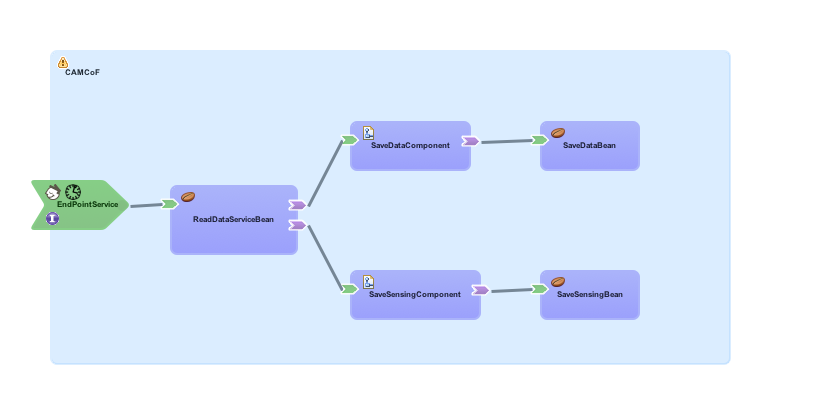
\includegraphics[scale=0.55]{Images/switchyard.png}
   \caption{Diagrama do SwitchYard com os componentes da arquitetura}
\end{figure}

\section{Interoperabilidade}

O desenvolvimento desta arquitetura está assente num princípio fundamental que se baseia em garantir a interoperabilidade de diferentes componentes. Com base neste princípio foram definidos e implementados métodos que permitem que diversos tipos de sensores possam efetuar de forma eficiente a sua ligação à arquitetura e assim contribuir para um correto funcionamento da plataforma. Posto isto é possível garantir não só uma comunicação transparente entre os diversos dispositivos, bem como uma troca efetiva de informação e permitir que novos sensores possam ser adicionados à arquitetura.

Antes de explicar em pormenor como é que esta arquitetura garante a interoperabilidade dos seus componentes, importa definir exatamente em que consiste a interoperabilidade e o que define um sistema com esta característica. Assim, a interoperabilidade é capacidade de diversos componentes comunicarem de forma transparente garantindo a cooperação entre eles. Estes componentes tem, em várias situações, origens tecnológicas e características bastante diferentes, o que leva a necessidade de definição de padrões de comunicação abertos e com recurso a linguagens e protocolos comuns(citação). Num sistema interoperável, como a arquitetura desenvolvida, todos os seus componentes devem então, independentemente da sua diversidade e definição tecnológica, ser capazes de cooperar e comunicar de forma clara e transparente através da definição de padrões e normas necessárias. A arquitetura implementada através dos padrões de comunicação definidos permite também a adição de forma automática de novos componentes, podendo estes acrescentar, através das suas funcionalidades, valor à arquitetura.(citações)

Posto isto, o método de ligação dos sensores, que podem ser vistos como os nodos da arquitetura responsáveis pela recolha de dados, à arquitetura foi definido de modo a garantir este conjunto de pressupostos apresentado. Foi então padronizado que os novos nodos para efetuarem a sua ligação à arquitetura devem enviar uma mensagem com um objeto JSON através do método POST para o seguinte endereço URL:

http://127.0.0.1:8080/CAMCoF/send/connect

O objeto a enviar pelo sensor que pretende conectar-se à arquitetura deve conter um conjunto de informações sobre o sensor de modo a que a arquitetura o consiga identificar e registar como um novo sensor da arquitetura. O objeto JSON deve assim conter o identificador do utilizador fornecido no momento de registo do utilizador na interface desenvolvida para a arquitetura, um endereço de comunicação do serviço para o qual a unidade central da arquitetura possa comunicar, um identificador do sensor, o tipo de serviço de monitorização oferecido pelo sensor, a frequência de comunicação de dados, o tipo de dados a enviar e ainda uma descrição do serviço.

\begin{lstlisting}[caption=Exemplo de objeto JSON enviado por Sensor de Teclado]
{
  "id": "1236",
  "ip": "23.254.109.135:999/keyboard/com",
  "type":"keyboard",
  "sensorid":"00:01:29:D3:95:C6",
  "period":"10",
  "typedata": "string",
  "description": "Keyboard Sensor Model A15526"
}
\end{lstlisting}

A unidade central perante a informação recebida inicia um processo de verificação da informação. Em primeiro lugar verifica se o identificador do sensor recebido corresponde a um sensor já utilizado na arquitetura, se não for este o caso o novo sensor será registado. Deste modo existe apenas um registo por cada sensor utilizado na arquitetura independentemente da sua utilização em vários momentos e do utilizador em questão. De seguida é registado o novo nodo da arquitetura, definido essencialmente pelo endereço de comunicação e pelo registo do sensor utilizado. Por fim, é criado o registo de monitorização ao qual serão associados os vários registos posteriormente levantados e enviados pelo nodo em questão.

\begin{figure}[htb]
   \centering
   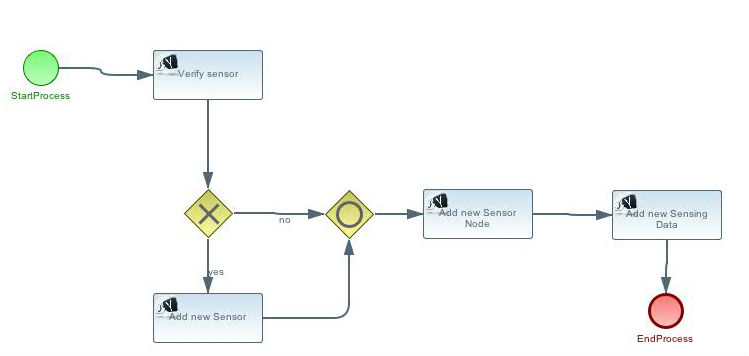
\includegraphics[scale=0.55]{Images/SaveSensingComponent.jpg}
   \caption{BPMN de conexão à arquitetura}
\end{figure}

Concluído este processo é enviada uma resposta ao pedido de conexão. Em caso de sucesso do pedido, independentemente do sensor já se encontrar registado previamente na arquitetura ou não, o novo nodo receberá como resposta um objeto JSON que será composto por um código de confirmação da integração do serviço na arquitetura e por um endereço através do qual o sensor deverá comunicar os dados a recolher durante a monitorização.\\

\begin{lstlisting}[caption=Mensagem de sucesso em JSON]
{
	"status":"200"
	"url":"http://127.0.0.1:8080/CAMCoF/send/1236/00:01:29:D3:95:C6"
}
\end{lstlisting}

No caso de se verificar algum problema com os dados enviados na mensagem de conexão à arquitetura, como por exemplo o identificador do utilizador não existir, ou de este nodo já se encontrar registado na arquitetura, a resposta obtida será uma mensagem a reportar o conflito ocorrido.\\

\begin{lstlisting}[caption=Mensagem de conflito em JSON]
{
	"status":"409"
	"url":"Conflict - Service already exists"
}
\end{lstlisting}


\section{Comunicação de Dados}

Definido o método de ligação dos nodos da arquitetura, importa estabelecer a forma como os dados recolhidos pelos sensores são enviados para a unidade central onde serão posteriormente tratados e armazenados. A comunicação da informação implementada na plataforma pretende garantir um método simples e fiável de transmissão dos dados de modo a que a informação possa ser gerida na unidade central. O feedback desta operação é também comunicada ao nodo da arquitetura responsável pela recolha da informação, para que este possa saber o estado deste processo em particular.

Na sequência do método implementado para a ligação dos nodos que compõem a arquitetura e de forma a garantir também os parâmetros básicos definidos para a comunicação da informação, esta operação estará exclusivamente disponível para os nodos conectados através do seguinte seguinte endereço URL:

http://127.0.0.1:8080/CAMCoF/send/id\_utilizador/id\_sensor

Este endereço foi definido de acordo com as informações registadas para cada nodo da arquitetura. Isto é, para cada nodo o \textit{id\_utilizador} irá corresponder ao identificador do utilizador registado na plataforma e o \textit{id\_sensor} ao identificador do sensor utilizado, informação essa registada no processo de conexão à arquitetura e já apresentado neste capítulo.

Relativamente aos dados a enviar estes são enviados sob a forma de uma String através do método POST. O exemplo abaixo representa um pequeno excerto de um registo de dados levantado por um sensor de movimento do rato sob a forma de uma String, que foi posteriormente enviada para a unidade central da arquitetura.\\
\begin{lstlisting}[caption=Excerto de dados levantado por sensor de movimento de rato]
MOV,63526767801398,None,599,36
MOV,63526767801404,None,600,36
MOV,63526767801416,None,601,36
MOV,63526767801436,None,601,36
MOV,63526767801480,None,602,36
MD,63526767801725,Left,602,36
MU,63526767801925,Left,602,36
\end{lstlisting}


Tendo em conta que este processo de comunicação da informação levantada pelos sensores é fundamental para o funcionamento da arquitetura, importa garantir que nenhum registo é perdido neste processo de comunicação. Posto isto, foi definido uma resposta padrão enviada pela unidade central para o nodo responsável pelo envio da informação dando conta do sucesso da operação. Assim, apenas no momento da receção dessa resposta o nodo poderá registar esse processo como concluído e avançar para a tarefa seguinte. Caso esta resposta não chegue, o nodo deve reenviar os dados para que esta possa ser registada. Abaixo apresenta-se o objeto JSON enviado pela unidade central dando conta do sucesso da operação de comunicação, como o próprio código presente no objeto indica.\\

\begin{lstlisting}[caption=Mensagem de sucesso em JSON]
{
	"code":"200"
}
\end{lstlisting}


Se a tentativa de comunicação for efetuada por um serviço que não se encontre, no momento, ligado à arquitetura o objeto de resposta contém o código 403, informando que este não tem permissões para estabelecer essa comunicação.


\section{Registo de Informação em bruto}

A informação recolhida pelos sensores que constituem a arquitetura deve ser armazenada para que seja possível, posteriormente, tratar os dados e retirar conclusões sobre estes. Deste modo, a informação que os sensores registados e conectados na arquitetura vão enviando para a unidade central é armazenada na base de dados antes de se iniciar qualquer tipo de operação sobre os dados. Nesta fase os dados são armazenados exatamente como foram registados pelos sensores, pelo que os registos correspondentes podem mais tarde ser consultados.

O armazenamento da informação em estado bruto na base de dados da plataforma representa  o primeiro nível de armazenamento de dados definido para o registo de informação proveniente dos sensores. Desta forma é possível ter, em qualquer momento, acesso à informação em bruto, caso esta seja necessária, avançando-se somente de seguida para o processamento dos dados com o recurso a serviços de métricas. 

O método de armazenamento dos dados implementado pretende assim o registo na base de dados da informação à medida que esta é enviada pelos nodos, em diferentes estados de tratamento, sendo esta primeira fase o início de um processo ao qual se segue o processamento da informação e posteriormente um novo registo da informação num outro nível. O objetivo deste método consiste em retirar o máximo de proveito da informação recolhida sobre o comportamento e ambiente em que o utilizador da arquitetura se encontra envolvido. 

\begin{figure}[htb]
   \centering
   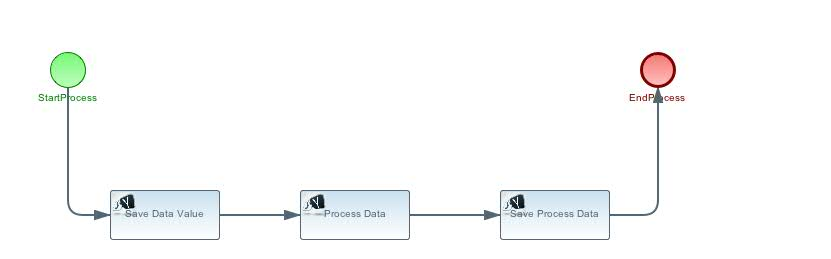
\includegraphics[scale=0.6]{Images/SaveDataComponent.jpg}
   \caption{BPMN de armazenamento da informação enviada pelos sensores}
\end{figure}

\section{Integração de Serviços de Métricas}

Os dados enviados pelos sensores para a unidade central e armazenados na base de dados em bruto são processados por um conjunto de serviços de métricas integrados na arquitetura, dando origem a um nível de informação mais refinado, sobre o qual se pretende conseguir retirar conclusões concretas. Os diversos serviços de métricas permitem que os dados recolhidos por um sensor de determinado tipo seja submetido a um processamento específico tendo em conta a sua origem. O resultado da execução dos serviços de métricas é novamente reencaminhado para a unidade central da arquitetura para que possa ser armazenado.

Assim à medida que os sensores recolhem informação e a encaminham para a unidade central, os dados recebidos são armazenados em bruto, tal como já foi explicado neste capítulo. De seguida, sempre que os serviços de métricas estejam disponíveis, são enviados para os serviços de métricas para que estes possam processá-los. Importa então sublinhar a forma como estas métricas foram desenvolvidas e integradas na arquitetura, bem como o valor que acrescenta ao seu funcionamento e ainda apresentar os diversos tipos de métricas existentes e a forma como estes se relacionam com os dados em bruto recolhidos.

\subsection{Desenvolvimento de Métricas}

\subsection{Tipos de Métricas - acabar preencher}

Os serviços de métricas disponíveis na arquitetura estão diretamente relacionados com o tipo de sensor responsável pela recolha de informação. Desta forma, para cada registo recolhido por um sensor, este poderá ser processado por diversas métricas desse tipo de dados, obtendo-se como resultado um registo correspondente a cada serviço de métrica utilizado. Cada métrica terá um foco específico, sendo o resultado obtido um registo do comportamento do utilizador nesse aspeto em concreto.

Posto isto, foram integrados na arquitetura um conjunto de tipos de métricas que pretendem  complementar a capacidade de agregação de informação da arquitetura, permitindo que esta possa ser analisada sob vários parametros e de diferentes formas. De seguida são então apresentados os tipos de métricas integradas na arquitetura neste momento, uma pequena descrição de cada métrica e ainda o tipo de dados a que cada uma se encontra associado.

\begin{center}
    \begin{tabular}{ | p{4cm} | l | p{7cm} |}
    \hline
    Nome & Tipo Dados & Descrição \\ \hline
    Key Down Time & Teclado & Tempo durante o qual uma tecla é pressionada. \\ \hline    		    Time Between Keys & Teclado & Tempo percorrido entre duas teclas pressionadas. \\ \hline
    Mouse Velocity & Rato & A distância percorrida pelo rato em pixels por intervalo de tempo, em milisegundos. \\ \hline
    Mouse Acceleration & Rato & A velocidade do rato em pixels/milisegundo por intervalo de tempo, em milisegundos. \\ \hline
    Time Between Clicks & Rato & Tempo percorrido entre dois cliques do rato. \\ \hline
    Double Click Duration & Rato & Tempo percorrido entre dois cliques seguidos, sempre que esse valor for inferior a 200 milisegundos. \\ \hline
    Average Excess of Distance & Rato & Calcula o excesso de distância médio percorrido durante um clique do rato. \\ \hline
    Average Distance of the Mouse to the Straight Line & Rato & Calcula a distância média percorrida em linha reta definida pela localização de dois cliques consecutivos. \\ \hline
    Distance of the Mouse to the Straight Line & Rato & Calcula a distância percorrida em linha reta definida pela localização de dois cliques consecutivos. \\ \hline
    Signed Sum of Angles & Rato & Pretende determinar se o movimento do rato tende a desviar mais para a direita ou para a esquerda. \\ \hline
    Absolute Sum of Angles & Rato & Pretende quantificar o desvio do movimento do rato independentemente da sua direção. \\ \hline
    Distance Between Clicks & Rato & Representa a distância total percorrida entre dois cliques consecutivos. \\ \hline
    \end{tabular}
\end{center}

Faltam aqui os dois do acelerometro e meter citacao 

\section{Comunicação com Serviços de Métricas}

Os serviços de métricas integrados são externos à arquitetura, contudo prestam um serviço bastante importante para o seu funcionamento. Através do método de comunicação estabelecido entre a unidade central da arquitetura e os diversos serviços de métricas, estes recebem os registos em bruto recolhidos pelos sensores e retornam esses dados processados de acordo com as métricas implementadas.

A comunicação estabelecida entre os serviços de métricas e a unidade central da arquitetura, baseia-se mais uma vez no envio de uma String correspondente aos dados registados na arquitetura, através do método POST. Tal como já foi referido, cada tipo de dados permitirá a utilização de um conjunto de métricas com as quais está relacionado. Desta forma, é também nesta fase que é feita a associação entre o tipo de sensor a que correspondem os dados recolhidos e consequentemente filtrado o conjunto de serviços de métricas a utilizar. Posto isto, são enviados os dados a processar para esse conjunto de métricas através do método de  comunicação descrito.

\begin{figure}[htb]
   \centering
   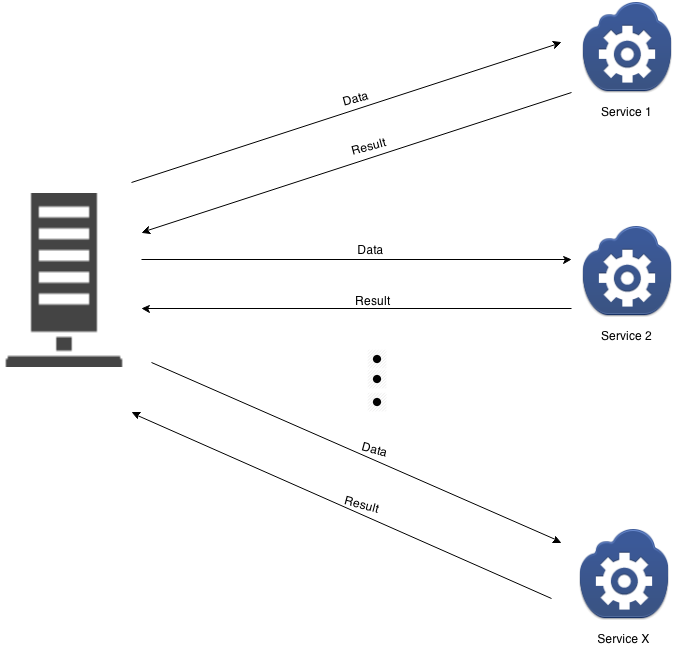
\includegraphics[scale=0.5]{Images/metricsdiagram.png}
   \caption{BPMN de armazenamento da informação enviada pelos sensores}
\end{figure}

Como resultado do processamento dos dados enviados cada serviço de métrica retorna um valor correspondente ao \textit{input} submetido. Estes dados processados de acordo com as métricas implementadas correspondem a um nível de informação mais refinado do que o anteriormente submetido. Sendo também este registado na base de dados da aplicação para posterior utilização.

\section{Registo de Informação Processada}

O registo da informação resultante da utilização dos serviços de métricas integradas na arquitetura corresponde a um nível de dados superior relativamente aos dados em bruto armazenados numa fase anterior. O armazenamento dos dois estados dos dados garante não só a consulta dos dados em bruto caso seja necessário, como garante que caso os serviços de métricas não estejam disponíveis em determinado momento, os dados possam ser submetidos para os serviços correspondentes posteriormente.

Este estado da informação é então armazenado na base de dados da aplicação, tal como no caso da informação em bruto, à medida que os serviços de métricas vão respondendo com a informação processada. Esta informação é armazenada como correspondente a um segundo nível de informação, que indica que esta se encontra refinada comparativamente ao primeiro nível, os dados em bruto. Nesta fase a informação registada pode ser agora utilizada como indicador de ocorrência de estados como fadiga ou stress por parte dos utilizadores da arquitetura.

\section{Verificação de Serviços Conectados}

A arquitetura pode em cada instante ter vários sensores conectados a recolher informação para a unidade central. Dada esta situação torna-se relevante haver um controlo sobre o estado em que se encontra cada um dos sensores ligados ao longo do tempo. Com esse intuito e de forma a haver uma gestão eficiente dos nodos da arquitetura foi pensada e desenvolvida uma forma de gerir e controlar o estado destas ligações com o decorrer do tempo.

Assim, tal como já foi abordado neste capítulo, à medida que cada sensor estabelece uma ligação à arquitetura, essa ligação para além de registada na base de dados, é também armazenada dinamicamente como um sensor que nesse instante se encontra ligado à arquitetura a recolher e transmitir novos dados. É sobre esse registo dinâmico que deve ser feito o controlo de ligação ao longo do tempo, para prevenir situações em que por algum motivo, ocorra um problema com um sensor e este pare de comunicar ou recolher informação, ou simplesmente termine o seu período de monitorização.

Para controlar a ocorrência destas situações foi estabelecido uma comunicação periódica entre a unidade central e todos os sensores que se encontram conectados nesse momento, de modo a confirmar se estes se mantém ligados à arquitetura. Para tal é enviada uma mensagem JSON através do método POST, para cada um dos nodos, na qual é indicado o identificador do utilizador, o identificador do sensor em questão e que se trata de um pedido de informação sobre o seu estado.\\

\begin{lstlisting}[caption=Mensagem de verificação de estado de um nodo]
{
	"id" : "1236",
  	"sensorid" : "00:01:29:D3:95:C6",
	"status" : "request"
}

\end{lstlisting}

O endereço de comunicação utilizado é o endereço URL fornecido por cada serviço no momento da conexão à arquitetura. Como resposta cada nodo deverá enviar um objeto JSON semelhante, contendo o atributo \textit{status} o código 200 caso este pretenda confirmar a permanência da conexão ou o código 410 caso esta pretenda terminar a ligação. Pode ainda ocorrer um terceiro cenário, no qual o nodo não responda em tempo útil, dando-se uma situação de \textit{timeout}, sendo o nodo eliminado da lista de serviços conectados nesse momento.

Todo este processo de verificação de serviços ligados à arquitetura é repetido de forma frequente e periódica pela arquitetura para garantir que não existe um acumular de serviços que já terminaram o seu período de monitorização, sem que a unidade central tenha conhecimento disso e possa por em causa o correto funcionamento da arquitetura.

\section{Conclusão}

O principal objetivo da arquitetura desenvolvida, tal como já foi abordado, consistia na construção de uma arquitetura que permitisse a recolha de informação através da utilização de sensores colocados de forma distribuída. Assim os sensores seriam capazes de monitorizar o comportamento dos utilizadores e permitir que esses dados fossem armazenados para posterior utilização e análise. Este objetivo, através das etapas percorridas e apresentadas neste capítulo, foi alcançado. A arquitetura desenvolvida permite que os seus utilizadores usem diversos dispositivos de recolha de informação, em diversos locais, contextos diferentes e fontes de informação diversificadas também. Através da utilização desta arquitetura, os seus utilizadores têm garantias de fiabilidade e estabilidade de todo o sistema e ainda métodos de comunicação que garantem o correto funcionamento da arquitetura, bem como o armazenamento dos dados recolhidos.

Uma das decisões tomadas, que teve grande influência no desenvolvimento da arquitetura, e que importa mais uma vez sublinhar foi a escolha da \textit{framework} SwitchYard para implementar a arquitetura. Esta decisão revelou-se extremamente sensata pois o potencial identificado na análise feita à \textit{framework} acabou por se verificar e foi bastante útil durante o período de desenvolvimento. O SwitchYard, orientado para o desenvolvimento de aplicações orientadas a serviços, permitiu, através do vasto leque de componentes que dispõe, definir um design e implementação da comunicação entre os nodos da arquitetura e a unidade central e desenvolver ainda as funcionalidades exigidas para essa unidade. Todo o processo de desenvolvimento beneficiou da utilização da \textit{framework}, podendo-se inclusivamente afirmar que este se revelou mais simples, orientado e rápido graças a este.

Outro dos aspetos a salientar nesta arquitetura é a sua comunicação e a forma como esta é estabelecida nas várias tarefas executadas ao longo de todo o processo ao qual a informação recolhida é sujeita. Os métodos de comunicação estabelecidos e implementados permitem garantir que todo o fluxo pelo qual a informação passa seja efetuado de forma eficiente e fiável. O cuidado no desenho destes métodos de comunicação teve ainda por base garantir a interoperabilidade de todos os componentes da arquitetura. Deste modo, é possível afirmar que a arquitetura oferece aos seus utilizadores a capacidade de utilizar diversos tipos de sensores sem que isto coloque em causa o seu correto funcionamento. Cada utilizador pode assim recorrer aos sensores que entender, dado que os métodos de comunicação implementados permitem uma ligação eficiente destes dispositivos e a sua cooperação na execução das suas tarefas no contexto da arquitetura.

De referir ainda a utilização dos serviços de métricas e do valor que acrescentam à arquitetura e ao serviço que oferecem aos seus utilizadores. Estas permitem que os dados recolhidos sejam refinados para um nível perceptível por parte dos utilizadores. Para além disso abrangem vários aspetos do comportamento do utilizadores monitorizados e permitem ter uma noção real dos registos e variações ocorridos ao longo do período de monitorização. Esta panóplia de informação que a arquitetura consegue oferecer, para determinados tipos de dados, acrescenta bastante valor à arquitetura. Para além disso, o método de comunicação e integração dos serviços de métricas está implementado de forma a que seja possível facilmente agregar e disponibilizar novos serviços de métricas, bastando para isso que estes novos serviços sejam registados na base de dados da arquitetura.



\chapter{Caso de Estudo}

Um dos objetivos desta dissertação passa por demonstrar a capacidade da arquitetura implementada em recolher e processar informação através da utilização de diversos tipos de sensores e apresentar resultados com origem nesses dados. Com esse intuito foi feito um caso de estudo sob diversas variáveis com o intuito de demonstrar a funcionalidade e interoperabilidade da arquitetura. Para tal foi definido um conjunto de sensores a utilizar, de forma a que da monitorização efetuada resultasse informação diversificada, foi selecionado o tipo de ambientes e situações de monitorização, para além do tipo de utilizadores escolhido para este caso de estudo. Foram ainda utilizadas os serviços de métricas integrados na arquitetura relacionados com os tipos de dados recolhidos, de forma a processar a informação e alcançar um nível de dados mais refinado. Tudo isto permitiu alcançar um conjunto de resultados que será apresentado neste capítulo, bem como todo os passos percorridos até alcançar esses resultados.


\section{Sensores Utilizados}

A escolha dos sensores a utilizar neste caso de estudo tiveram por base várias razões e condicionantes de acordo com o objetivo a alcançar com esta demonstração em particular. Tendo esta experiência como principal intuito demonstrar a funcionalidade da arquitetura e a sua interoperabilidade, a escolha dos sensores foi ponderada nesse sentido. Pretende-se então neste caso utilizar dispositivos fiáveis, baseados em tecnologias diferentes e capazes de recolher diferentes tipos de dados. Para além disso, a facilidade de acesso aos dispositivos, o comportamento dos utilizadores no contexto a monitorizar e ainda os serviços de métricas integrados na arquitetura, foram outros pontos a tidos em consideração. Foi sob este fatores que foi selecionado um conjunto de sensores que se pretende que cumpram os requisitos definidos.

Com base neste conjunto de fatores e tendo em conta a importância de cada um foram selecionados três tipos de sensores para esta demonstração: rato, teclado e acelerómetro. Estes três tipos de sensores, em primeiro lugar, são sensores aos quais era possível aceder com relativa facilidade e de simples utilização para os seus utilizadores. Este tipo de equipamento são equipamentos muito utilizados em diversos contextos e há bastante tempo. Isto confere-lhe um nível de desenvolvimento e robustez que garante um pressuposto fundamental nesta escolha que diz respeito à fiabilidade do equipamento e da informação recolhida. O facto do conjunto de sensores escolhido ser composto por três tipos de sensores corresponde a um número aceitável de opções, o que levará a um número de serviços de métricas a utilizar alargado. O que consequentemente permite um nível de diversidade de informação suficiente para demonstrar a funcionalidade da arquitetura desenvolvida.

Outro fator fundamental na seleção deste três tipos de sensores prende-se com o comportamento e contexto de monitorização por parte dos diferentes utilizadores neste caso de estudo. Esta demonstração pretende, como base de recolha de informação, extrair informação sobre comportamento dos seus utilizadores e da sua interação com o computador como ferramenta de trabalho ou de lazer. Com base neste objetivo, a utilização deste três tipos de sensores enquadra-se perfeitamente dado que incidem sobre os dispositivos mais comuns usados pelos utilizadores para interagir com a máquina. Para além disso os \textit{gateways} de comunicação dos sensores escolhidos para a demonstração são baseados em tecnologias diferentes. No caso dos sensores de rato e teclado são baseados em C\#, enquanto que no caso do acelerómetro é baseado em Java. Desta forma, a capacidade de cooperação destes sensores na arquitetura permitirá também demonstrar a sua interoperabilidade.

O conjunto de fatores e correspondentes decisões tomadas, que levaram à escolha da seleção de sensores apresentada, garantem os pressupostos necessários para cumprir os objetivos pretendidos com este caso de estudo. Desta forma foram reunidas condições que permitirão alcançar resultados que demonstrem a funcionalidade, interoperabilidade e ainda a utilidade da arquitetura para os seus utilizadores.

\section{Tipos de Utilizadores}

Na construção de um caso de estudo existem várias questões a ponderar. Neste em particular em que um dos objetivos é demonstrar a funcionalidade e utilidade da arquitetura desenvolvida, a escolha dos utilizadores é uma parte fundamental. Deve então ser ponderado qual o perfil de utilizadores para a demonstração e atentar na sua diversidade. Deste modo, importa garantir que o conjunto de utilizadores escolhidos para a recolha de dados através da utilização da arquitetura apresentam diferentes características com o intuito de acrescentar solidez aos resultados finais e assim conseguir obter conclusões mais claras.

Com base neste pressuposto, foram ponderadas todas as características da arquitetura apresentadas para definir um conjunto de utilizadores adequado ao objetivo deste caso de estudo. Posto isto, foi definido um conjunto de três utilizadores com diferentes interesses, diferentes características pessoais, e ainda com personalidades distintas. Com esta opção pretende-se aumentar a probabilidade de verificar resultados distintos para os vários parâmetros a analisar, apesar do recurso ao mesmo tipo de aparelhos de monitorização.

Foram então escolhidos três pessoas para testar a arquitetura através da utilização dos três tipos de sensores apresentados. Dois utilizadores têm 24 anos e outro tem 26 anos de idade. Todos eles são pessoas ligadas à área da informática, estando a sua vida profissional diretamente ligada à utilização de computadores, sendo assim possível recolher informação sobre todos em diversos contextos de utilização. Todos eles têm personalidades distintas, um é uma pessoa extremamente calma e ponderada, o segundo é obcecado pelo trabalho, dedicando-lhe grande parte do seu tempo, e o terceiro trata-se de uma pessoa bastante impulsiva e normalmente bastante stressada. A diversidade de personalidades e perfil das pessoas escolhidas aliadas à possibilidade de todos serem monitorizados em diferentes ambientes mas que lhes são naturais e familiares permitem a diversidade de condicionantes pretendida para este caso de estudo.


\section{Ambientes de Teste}

Depois de definidos os tipos de utilizadores e meios tecnológicos para construir o caso de estudo, falta analisar quais os tipos de contextos mais adequados para efetuar a recolha de informação. A definição destes contextos deve ter em conta que, naturalmente, existem situações cuja tendência a ocorrer determinados tipos de reação é mais propícia do que noutras. Por exemplo, no caso da monitorização ocorrer num ambiente de trabalho, a tendência a verificar-se resultados que possam indiciar stress ou fadiga com o passar do tempo é bastante mais provável do que verificar-se esses indícios em situações de lazer ou divertimento.

Posto isto, deve ser definido um conjunto de ambientes e contextos durante os quais os utilizadores selecionados devem, de forma menos intrusiva possível, ser monitorizados. Pretende-se desta forma garantir que a utilização de sensores, para a recolha informação, interfira o mínimo possível com o normal comportamento das utilizadores, independentemente do ambiente em que este se encontra no momento. Sendo que os sensores definidos para este caso em particular têm essa particularidade. Para além disso, os ambientes de teste definidos devem ser iguais para todos os utilizadores e também diversificados. Ou seja, todos os utilizadores devem ser sujeitos aos mesmos tipo de ambientes e às mesmas condições de modo a que seja possível comparar os diferentes resultados entre estes. Deve também ser definido um conjunto de ambientes suficientemente amplo de modo a que situações distintas possam ser analisadas e comparados resultados entre ambientes cujas diferenças sejam percetíveis.

Tendo em conta a relevância de todos os pontos já descritos foram escolhidas três situações para a recolha de informação neste caso de estudo. A primeira situação escolhida foi o ambiente de trabalho, em que os utilizadores, todos eles sujeitos à utilização do computador no seu período de trabalho, estão constantemente a ser monitorizados durante largos períodos de tempo. Esta situação é muito específica pois tratam-se de ambientes normalmente intensos, desgastantes e por vezes de grande stress para os utilizadores, sendo provável a ocorrência de comportamentos que revelem indicações nesse sentido. A segunda situação definida foi a utilização livre da Internet, ou seja, trata-se de um ambiente fora do âmbito de trabalho em que o utilizador navega normalmente na Internet de forma livre. Trata-se portanto de uma situação de lazer e descanso para o utilizador. O terceiro e último ambiente de utilização definido foi a utilização do Facebook, dado que é uma rede social de ampla utilização, em que todos os utilizadores se sentem familiarizados e em que normalmente passam muito do seu tempo diário. A utilização do Facebook está atualmente bastante ligada com a vida pessoal e social das pessoas, dada a forma como as pessoas normalmente a utilizam e envolvem na sua vida. Desta utilização podem resultar comportamentos e resultados bastante interessantes por parte dos utilizadores durante a monitorização.

\begin{figure}[htb]
   \centering
   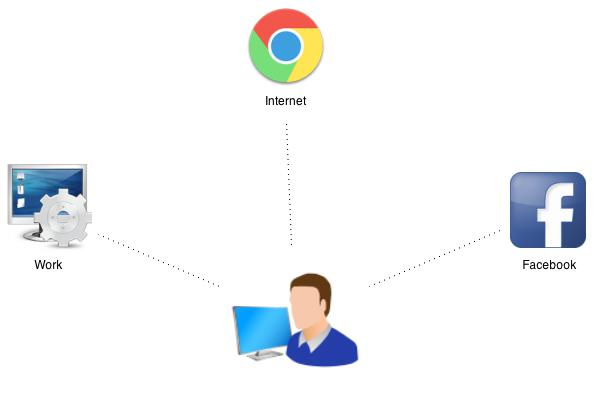
\includegraphics[scale=0.5]{Images/ambientesestudo.jpg}
   \caption{Ambientes de teste definidos}
\end{figure}

\section{Serviços Utilizados}

A decisão sobre os serviços de métrica a utilizar neste caso de estudo esteve diretamente ligada aos sensores escolhidos e consequentemente ao tipo de dados recolhidos. Tal como já foi explicado a escolha dos sensores teve como um dos parâmetros a ter em conta a possibilidade de utilização de um grande número de métricas, pelo valor que estas acrescentam ao trabalho, mas também relativamente aos resultados que é possível obter.

Tendo por base estes aspetos, e tendo em conta que os sensores escolhidos para este caso de estudo foram sensores de rato, teclado e o acelerómetro, é possível utilizar todos os serviços de métricas integrados na arquitetura e apresentados no capítulo anterior. A utilização desta panóplia de serviços irá permitir alcançar um conjunto diversificado de indicadores, num nível de informação acima dos dados em bruto e deste modo enriquecer os resultados deste caso de estudo.

\section{Resultados}

O caso de estudo efetuado teve por base todas as decisões tomadas e explicadas neste capítulo. Isso permitiu definir um conjunto de pressupostos com o intuito dos resultados do estudo demonstrarem a funcionalidade, interoperabilidade e utilidade da arquitetura desenvolvida, que é o seu principal objetivo. Pretende-se ainda apresentar diferenças percetíveis entre os resultados de monitorização dos utilizadores nos diversos momentos e ambientes definidos para este caso em particular. Desta forma serão apresentados os resultados alcançados, sublinhando determinados pontos e conclusões mais relevantes dado que o conjunto total de informação recolhido é bastante extenso.

Entre os diversos serviços de métricas integrados na arquitetura e utilizados neste caso de estudo resultaram grandes blocos de informação cujos resultados se revelaram bastante úteis e esclarecedores em diversos aspetos. De forma a analisar os resultados alcançados serão apresentados nesta secção análises comparativas no que diz respeito aos três utilizadores deste caso de estudo nas três tarefas definidas. Os resultados apresentados nesta secção foram selecionados por serem representativos da generalidade dos resultados alcançados, mas também por demonstrarem algumas características que se pretendia provar nesta experimentação.

Posto isto, e tal como já foi apresentado, este caso de estudo foi feito por três utilizadores com diferentes características de forma a analisar o seu comportamento em diversos parâmetros na execução de três tarefas diferentes. Uma dessas tarefas corresponde à utilização do Facebook. Neste aspeto o serviço de métricas que revelou resultados mais interessantes foi  o \textit{Key Down Time}. Este serviço de métrica, que corresponde aos dados recolhidos pelo sensor de teclado, apresenta o tempo durante o qual uma tecla é pressionada. A análise dos dados recolhidos e processados permite concluir que os três utilizadores apresentaram resultados bastante distintos.


O primeiro utilizador foi o que apresentou valores mais elevados revelando uma média correspondente ao dobro do segundo utilizador e muito superior ao terceiro utilizador. O terceiro utilizador revelou-se, de longe, o que menos tempo pressionava as teclas. Para além disso, a análise gráfica permite concluir que este último foi o mais constante entre os três utilizadores. O segundo utilizador apresenta também dados relativamente constante apesar de, no geral, serem mais elevados. O primeiro utilizador revelou-se o mais instável neste particular, registando-se várias variações durante o período de monitorização. O facto da variação das médias ser tão acentuado prende-se sobretudo com a ocorrência de variações pontuais dos registos que atingem valores extremamente altos. Apesar de algumas dessas variações serem percetíveis nos gráficos apresentados, a maioria dos casos tratam-se de situações pontuais e por isso não são visíveis.


\begin{figure}[htb]
   \centering
   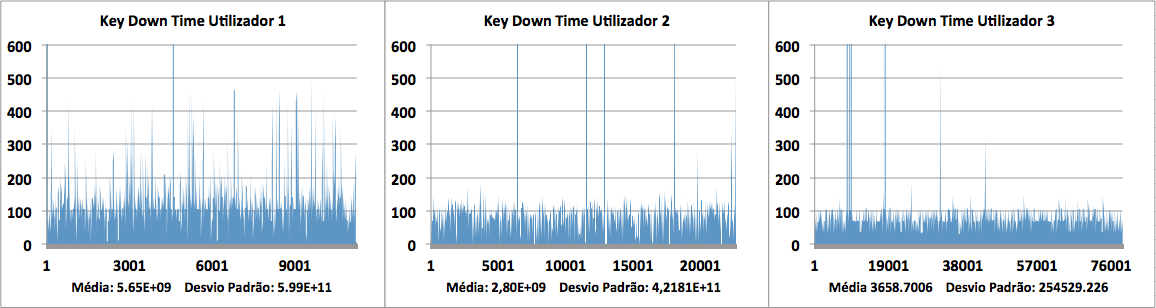
\includegraphics[scale=0.35]{Images/keydowntime11.png}
   \caption{Gráficos de resultados de Key Down Time dos três utilizadores na utilização do Facebook}
\end{figure}

A navegação de forma livre na Internet por parte dos utilizadores foi outro dos ambientes de monitorização ao qual estes foram sujeitos. No que diz respeito aos resultados obtidos através dos serviços de métricas importa realçar os resultados do \textit{Time Between Keys}. Esta métrica, também referente aos dados provenientes da utilização do teclado, representa o tempo percorrido entre duas teclas pressionadas. Neste aspeto o primeiro utilizador revelou-se o utilizador com o comportamento mais intenso, tal como indica o seu tempo médio. A análise gráfica dos seus resultados permitem ainda verificar que este se revelou o utilizador com menor número de variações significativas durante o seu período de utilização da Internet, nesta componente em particular. O segundo e terceiro utilizadores já revelaram um elevado número de variações acentuadas no que ao seu comportamento diz respeito. Para além disso, tiveram médias de tempo percorrido entre duas teclas pressionadas superiores, especialmente o segundo utilizador, apresentando já uma diferença significativa para o primeiro utilizador.

\begin{figure}[htb]
   \centering
   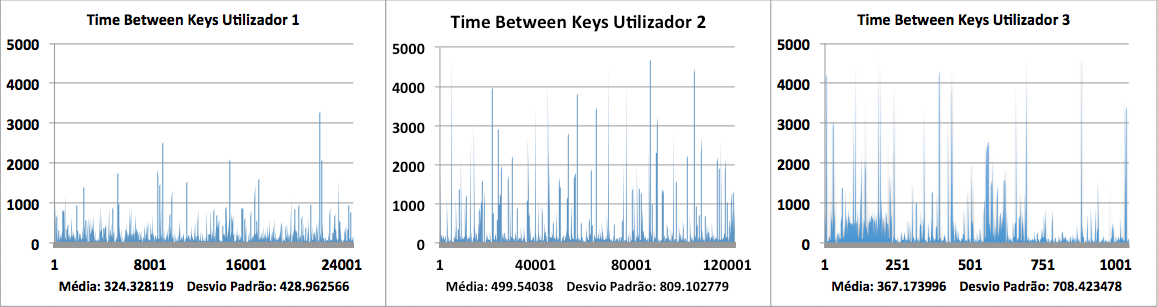
\includegraphics[scale=0.35]{Images/timebetweenkeys1.png}
   \caption{Gráficos de resultados de Time Between Keys dos três utilizadores na utilização da Internet}
\end{figure}

Estes resultados indicam uma escrita mais rápida por parte do primeiro utilizador e no sentido oposto uma escrita menos constante mas mais pausada por parte do segundo utilizador. Para além disso, sublinhar que este contexto de monitorização é o contexto escolhido de maior liberdade para o utilizador da arquitetura neste caso de estudo.

O outro contexto de monitorização definido foi o período de trabalho dos utilizadores. Este contexto normalmente é o mais intenso e desgastante dos três. De forma a poder comparar o desempenho dos três utilizadores neste ambiente são apresentados o resultados dos utilizadores correspondentes à velocidade do rato durante este período. Neste caso, os valores apresentados demonstram um cenário praticamente oposto aos resultados de monitorização apresentados para a utilização da Internet.

 \begin{figure}[htb]
   \centering
   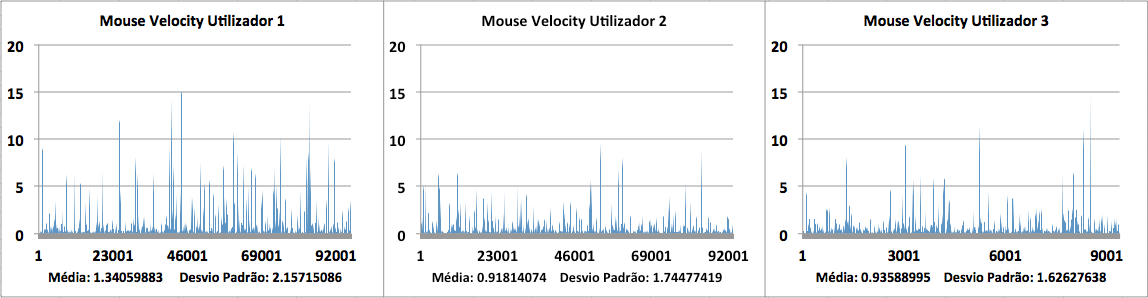
\includegraphics[scale=0.363]{Images/mousevelocity1.png}
   \caption{Gráficos de resultados de Mouse Velocity dos três utilizadores durante o período de trabalho}
\end{figure}

Os resultados do segundo utilizador demonstram que este foi o mais calmo, relativamente ao movimento do rato, durante o seu período de trabalho, registando-se também variações menos acentuados nos seus registos relativamente aos restantes utilizadores. O terceiro utilizador teve resultados próximos do segundo, revelando apenas um ligeiro aumento na sua média, tendo algumas variações mais acentuadas mas ainda assim um desvio padrão inferior ao segundo utilizador. Por fim, o primeiro utilizador foi o que apresentou resultados mais elevados, o que indica maior intensidade no seu período de trabalho comparativamente com os restantes utilizadores. A média de resultados apresentada pelo primeiro utilizador é superior aos restantes, bem como o seu desvio padrão e valores alcançados em determinados registos. De salientar ainda que o utilizador indicado neste capítulo como uma pessoa extremamente trabalhadora foi o segundo, contudo estes resultado demonstram que foi o mais calmo dos três neste contexto.



Outra análise relevante que deve ser tida em conta é a comparação de resultados obtidos pelo mesmo utilizador na execução de diferentes tarefas. Esta comparação permitirá verificar a diferença de comportamento de um utilizador sob condições diferentes e retirar conclusões sobre esses factos. Posto isto, foram selecionados os resultados do segundo utilizador para a métrica de \textit{Absolute Sum of Angles} que permite quantificar o desvio do movimento do rato independentemente da sua direção. Os resultados desta métrica, teoricamente, terá tendência a apresentar valores mais altos em situações de maior desgaste ou stress, por exemplo.

Os resultados obtidos desta forma apresentam diferenças significativas entre a monitorização efetuada durante a utilização do Facebook e Internet em relação à monitorização durante o período de trabalho. Os valores obtidos durante os dois primeiros contextos apresentam valores bastante semelhantes, tanto para os valores médios e desvios padrões como é inclusivamente visível graficamente. Esta semelhança de valores indica que em ambas as situações o segundo utilizador teve comportamentos semelhantes neste parâmetro em particular. Já no que diz respeito ao período de trabalho as diferenças são bastante acentuadas. A média e desvio são bastante superiores, sendo até necessário utilizar uma escala bastante maior para fazer a representação gráfica destes valores. 

 \begin{figure}[htb]
   \centering
   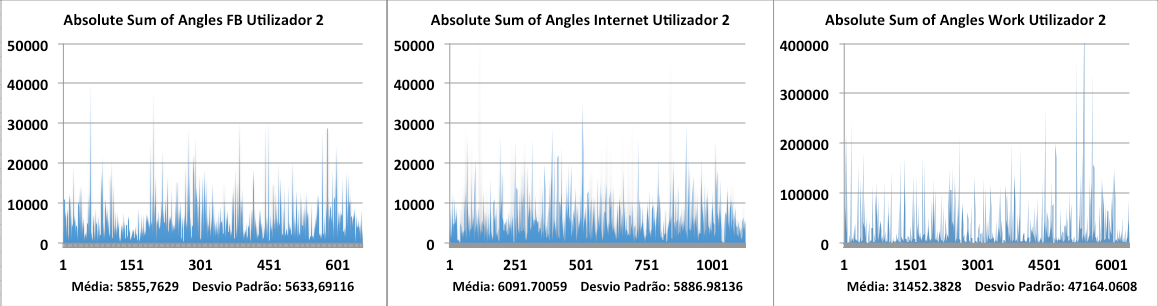
\includegraphics[scale=0.35]{Images/sumofangles1.png}
   \caption{Gráficos de resultados de Absolute Sum of Angles das três tarefas realizados pelo segundo utilizador}
\end{figure}

Estes valores demonstram de facto uma diferença acentuada entre duas situações de lazer, navegar na Internet e utilização de Facebook, relativamente a uma situação de trabalho com toda a carga que este contexto implica. O facto de ser um contexto mais pesado e com maior probabilidade de existência de situações como a fadiga e stress, justifica a variação de resultados entre os contextos analisados neste caso particular.


A utilização de acelerómetro neste caso de estudo não foi tão profunda e abrangente como a dos restantes sensores. A sua utilização não foi orientada às três tarefas definidas mas apenas num contexto livre por dificuldade de acesso ao próprio dispositivo, e apenas por dois utilizadores. Ainda assim, importa apresentar alguns resultados da sua utilização. Este tipo de dados também não tem, de momento, serviços de métricas desenvolvidos, contudo a análise dos seus resultados permite observar dados interessantes. Este tipo de sensor permitem verificar a aceleração ocorrida sobre três eixos, ou seja, permite obter a aceleração na diagonal, horizontal e vertical.

Os acelerómetros foram utilizados sobre as pernas, rato, teclado e cadeiras dos seus utilizadores de forma a tentar abranger vários pontos corporais e de interação com o computador. Os resultados apresentados correspondem aos dados recolhidos sobre a aceleração do primeiro utilizador sobre o seu movimento na cadeira. Como é possível verificar, os resultados indicam uma aceleração positiva tanto na horizontal como na diagonal, ao contrário da aceleração verificada na vertical que indica que o movimento neste eixo tem uma variação de velocidade negativa. De referir ainda que a aceleração na horizontal é a mais acentuada e a aceleração na diagonal regista alguns picos negativos, para além de ser a menos estável.

 \begin{figure}[htb]
   \centering
   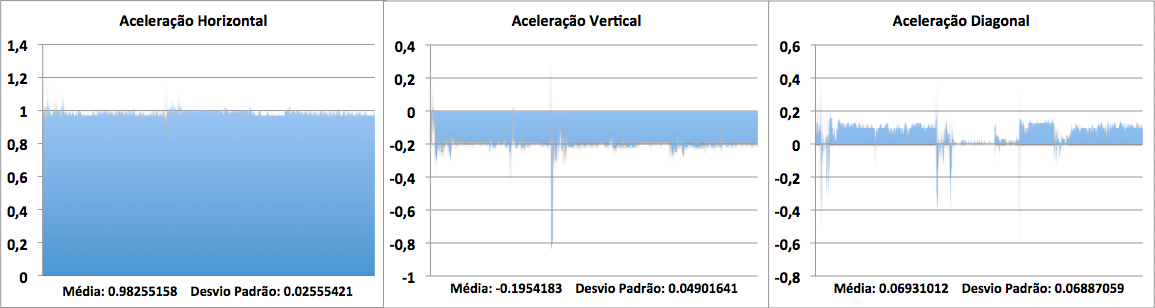
\includegraphics[scale=0.35]{Images/aceleracao1.png}
   \caption{Gráficos de resultados de acelerómetro sobre o movimento na cadeira}
\end{figure}



\section{Conclusão}

Este caso de estudo permitiu confirmar que a arquitetura desenvolvida é funcional e bastante útil para os seus utilizadores. Foi possível verificar que se trata de uma arquitetura com um funcionamento estável e cujas suas características e funcionalidades permitem uma recolha, tratamento e gestão da informação dos utilizadores fiáveis. A apresentação de diversos resultados e consequente análise do comportamento dos utilizadores efetuada neste capítulo demonstra que se trata de uma arquitetura com grande utilidade. A sua utilização em situações de monitorização, independentemente do contexto e localização dos dispositivos de recolha de informação, dá assim garantias de fiabilidade aos seus utilizadores.

Um fator importante para o sucesso deste caso de estudo foi o cuidado na escolha e definição de todos os parâmetros definidos para a experiência. A escolha de utilizadores com diferentes características, sob diferentes contextos de monitorização e ainda a seleção dos sensores a utilizar e consequentes serviços de métricas, confirmaram-se acertadas e contribuíram para a qualidade dos resultados. De menos positivo apenas salientar o facto da utilização do acelerómetro não ter sido tão abrangente quanto era pretendido. Para além disso, salientar ainda a demonstração de interoperabilidade da arquitetura. A utilização de sensores cujos \textit{gateways} são baseados em tecnologias diferentes demonstra a capacidade dos métodos de comunicação implementados e de componentes com diferentes bases tecnológicas serem capazes de cooperar com sucesso.

Relativamente ao conteúdo dos resultados alcançados, estes foram bastantes satisfatórios. Para além de provarem a funcionalidade da arquitetura, permitiram verificar vários pontos e situações muito interessantes no que diz respeito ao comportamento dos utilizadores. De referir ainda que, num cômputo geral, os resultados alcançados foram de encontro ao que se pretendia na definição prévia de todas as características pensadas para este caso de estudo. Ou seja, todas as condições do caso de estudo foram definidos de modo a que os resultados permitissem verificar algumas diferenças entre os contextos e resultados de cada utilizador. A análise final dos resultados demonstrou a existência dessas diferenças tal como se pretendia.

Outra conclusão retirada deste caso de estudo foi a utilidade dos serviços de métricas integrados na arquitetura. A utilização destes serviços na arquitetura permitiu analisar vários aspetos em particular e apresenta-los ao utilizador final, como estes resultados aqui apresentados demonstram. De assinalar ainda a diversidade de parâmetros e resultados obtidos através desta experiência. Apesar de apenas terem sido utilizados três tipos de sensores e três utilizadores, para além das restantes condições definidas para este caso em particular, os resultados obtidos foram bastante abrangentes. Foi possível obter resultados de um número bastante alargado de aspetos e analisar o comportamento de cada utilizador nesses contextos. 

\chapter{Interface Web}

Com arquitetura desenvolvida e disponível os seus utilizadores devem ter uma plataforma através da qual consigam acompanhar os registos provenientes da sua utilização da arquitetura. Esse é também um dos objetivos desta dissertação, ou seja, desenvolver uma interface através da qual cada utilizador consiga aceder aos seus dados e às várias informações relacionados com a monitorização efetuada através da solução desenvolvida. Serão apresentados neste capítulo a metodologia de desenvolvimento utilizada na conceção da interface web, os diferentes níveis de acesso existentes na plataforma, bem como as funcionalidades disponíveis para cada cada tipo de utilizador e ainda um conjunto de conclusões sobre a interface implementada.

\section{Padrão de Desenvolvimento}

No desenvolvimento da plataforma Web, através da qual os utilizadores poderão aceder aos seus registos de monitorização, o padrão de arquitetura de software utilizado foi o MVC. Este padrão, cuja sigla MVC signfica \textit{Model-View-Controller}, trata-se de um dos padrões de desenvolvimento de software mais utilizados atualmente, e tem por base promover a reutilização do código desenvolvido, bem como a separação de conceitos e definição de interação entre eles em termos de arquitetura de software\cite{bucanek2009model}. 

Este torna-se extremamente útil, e consequentemente bastante utilizado, com o aumento da complexidade das aplicações a desenvolver. Este facto levou a que existisse a necessidade de separar conceitos de forma a simplificar o processo de desenvolvimento para os responsáveis pela construção destas plataformas. Deste modo, torna-se fundamental a separação entre os dados da aplicação e a camada de apresentação, garantindo assim que as alterações feitas no \textit{layout} não interferem com a manipulação dos dados e que estes podem ser modificados sem que isso tenha repercussões no \textit{layout}. Esta separação apenas é possível pela existência de um componente responsável pela intermediação entre os dois, o controlador\cite{bucanek2009model}.

O modelo MVC, utilizado no desenvolvimento desta interface Web, divide assim os componentes da aplicação em três camadas: o \textit{Model} que representa os dados e o métodos de acesso e edição destes, a \textit{View} que corresponde à camada de visualização da aplicação, sendo a parte responsável pela iteração com os utilizadores. E por fim o \textit{Controller} que contém os métodos que processam os pedidos provenientes da \textit{view} e pode também invocar alterações no \textit{model}, funcionando como um controlador da aplicação e a ponte entre as duas camadas restantes. Desta forma é possível organizar de forma mais modular a arquitetura de uma aplicação web, centrando em cada camada única e exclusivamente as funções para as quais essa foi concebida, simplificando estruturalmente o desenvolvimento da aplicação.

\section{Tipos de Acesso}

A interface web criada para complementar a utilização da arquitetura foi desenhada com dois níveis de acesso para os seus utilizadores. Desta forma, os dois tipos de perfis existentes terão permissão de acesso a diferentes funcionalidades e informações da plataforma. Esta divisão de permissões em apenas dois níveis baseia-se na necessidade de ter um acesso para o utilizador comum consultar as suas informações e registos, e outro acesso para que o administrador possa consultar todos os conteúdos de administração relevantes da plataforma.

O acesso com maior nível corresponde assim às permissões de administração. Este nível de acesso disponibiliza um conjunto alargado de informações sobre os utilizadores da arquitetura, dos registos de monitorização efetuados e ainda sobre os sensores conectados à arquitetura bem como o seu funcionamento. Este perfil de utilizador corresponde ao tipo de acesso mais elevado definido para esta interface e apenas um conjunto restrito de utilizadores devem ter acesso a estes conteúdos.

 \begin{figure}[htb]
   \centering
   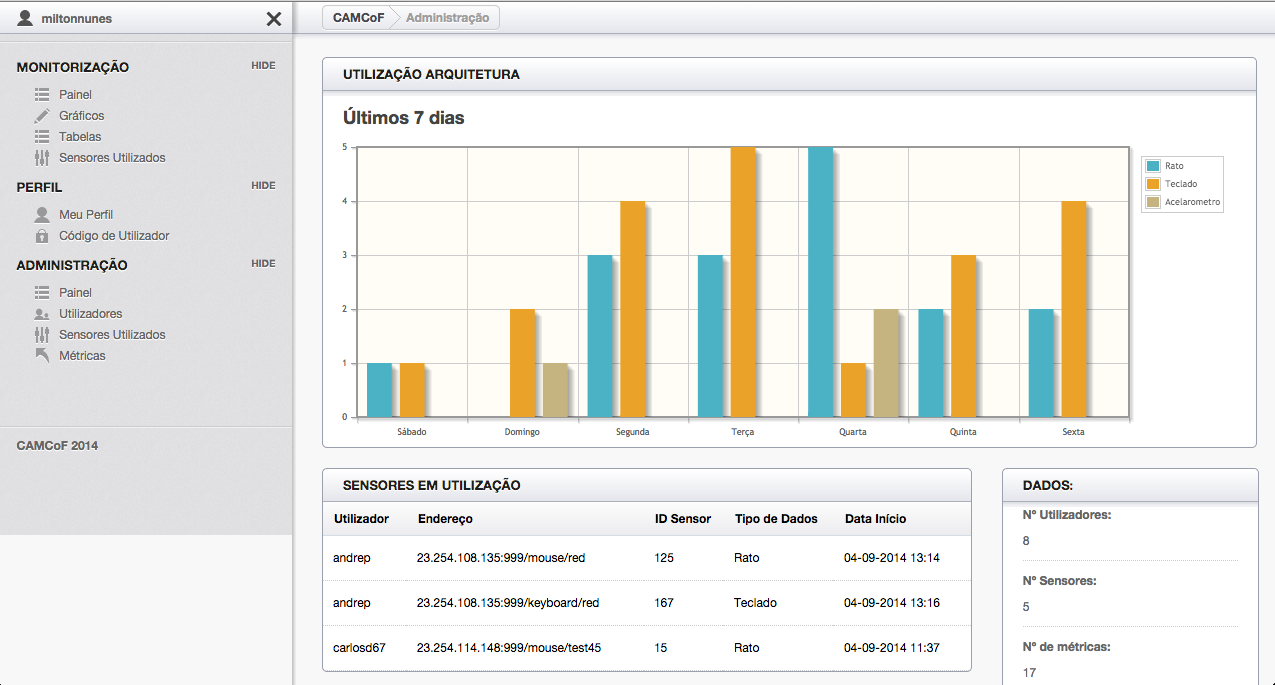
\includegraphics[scale=0.29]{Images/panel.png}
   \caption{Página principal de Administrador}
\end{figure}

O outro nível de acesso implementado corresponde ao acesso atribuído aos utilizadores comuns da arquitetura. Através do seu acesso à interface os utilizadores da arquitetura conseguem aceder às suas informações pessoais e a todos os dados relacionados com a sua monitorização. Deste modo, tem acesso a todos os seus registos de monitorização apresentados de diferentes formas e pode ainda efetuar consultas sobre todo o seu histórico. Este nível representa um acesso mais restrito que o anterior, visto que limita os dados apresentados apenas aos correspondentes ao próprio utilizador e aos seus registos de monitorização.

 \begin{figure}[htb]
   \centering
   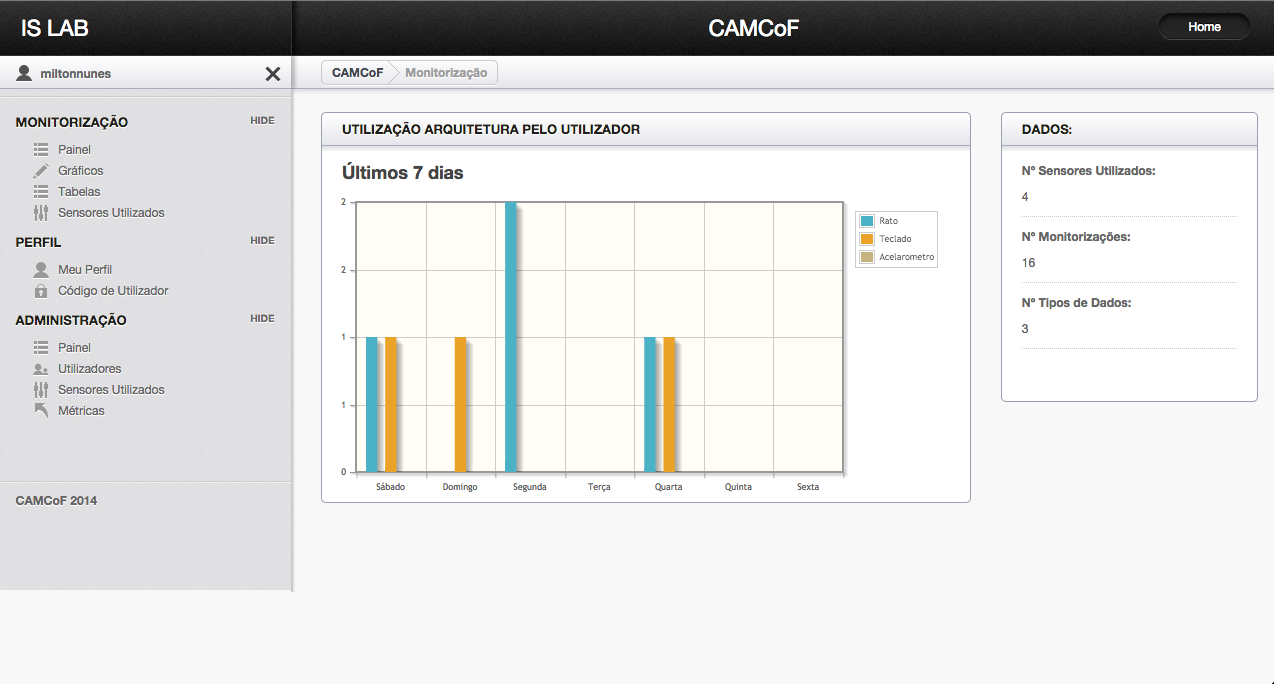
\includegraphics[scale=0.29]{Images/home.png}
   \caption{Página principal de Utilizador}
\end{figure}

\section{Funcionalidades de Utilizador}

No contexto de utilização da arquitetura por parte de um utilizador, é extremamente importante este poder consultar e analisar os resultados da sua monitorização. Deste modo, um dos objetivos no desenvolvimento da interface foi fornecer aos utilizadores acesso a todo o seu histórico de registos provenientes da utilização da arquitetura desenvolvida. Cada utilizador terá assim na sua área pessoal acesso total a todo o conteúdo de informação recolhida e processada pela arquitetura. Para além disso terá ainda disponível diversas formas de acesso e apresentação da informação, com o intuito de que os seus utilizadores possam tirar o máximo de proveito dos seus próprios dados.

Assim para além das informações mais genéricas apresentados a cada utilizador na sua página principal, este poderá aceder a duas áreas da interface nas quais poderá consultar todos os seus registos de monitorização. A diferenças entre estas duas áreas reside na forma de apresentação da informação. Na primeira área o utilizador poderá aceder aos seus registos sob a forma de tabela, selecionando o tipo de dados que pretende consultar e uma métrica associada ao tipo de dado escolhido. No caso de esse tipo de dados não conter nenhuma métrica disponível na arquitetura a informação será apresentada em bruto, tal como foi recolhida pelo dispositivo responsável pela monitorização. Para além disso, o utilizador poderá ainda escolher o período de monitorização que pretende, tendo em conta obviamente os dois parâmetros já definidos.

 \begin{figure}[htb]
   \centering
   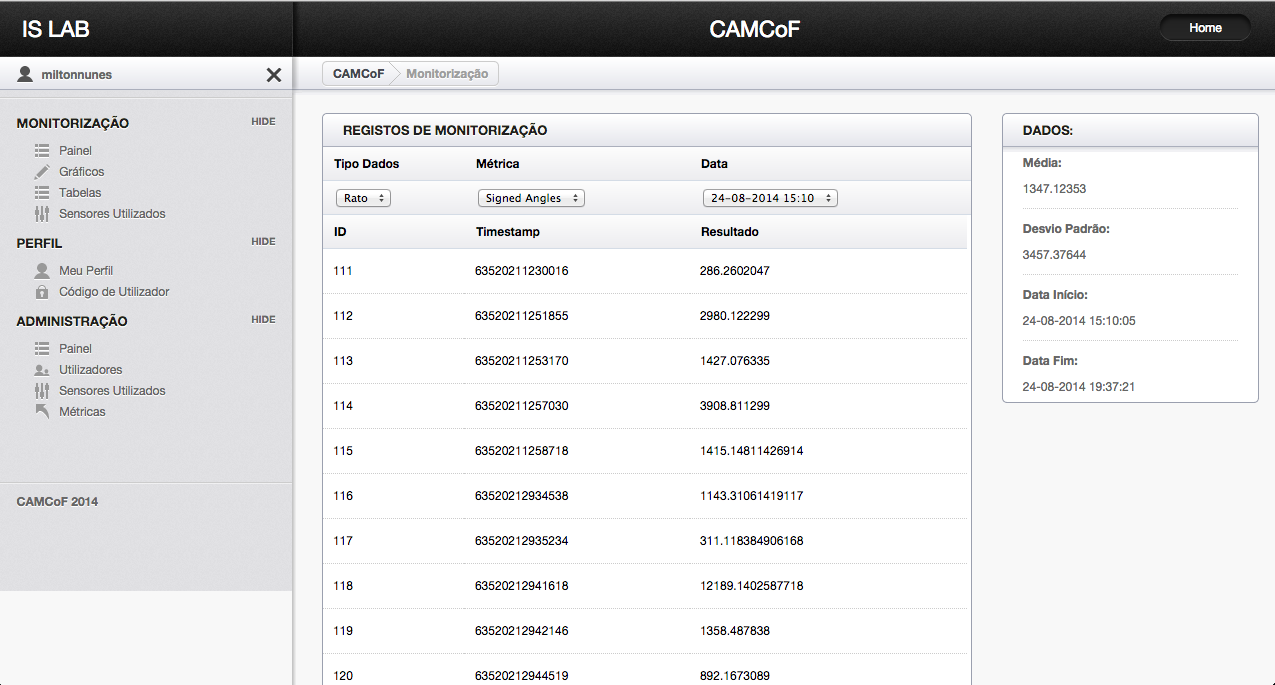
\includegraphics[scale=0.29]{Images/tables.png}
   \caption{Página de visualização de registos de monitorização sob a forma de tabelas}
\end{figure}

A segunda área de apresentação dos registos de monitorização disponibilizada trata-se da apresentação de resultados através de gráficos. Esta forma de apresentação é bastante útil para os utilizadores pois permitem-lhe ter uma noção gráfica mais clara dos seus registos e variações comportamentais ao longo do período de monitorização. Esta área oferece assim uma forma mais simples de visualização e interpretação dos resultados. Tal como na área composta por tabelas, o utilizador poderá selecionar o tipo de dados, uma métrica associada e a data do período a visualizar. Neste caso em particular apenas os tipos de dados com métricas associadas serão apresentados devido à dificuldade em gerar gráficos através de informação em bruto.

 \begin{figure}[htb]
   \centering
   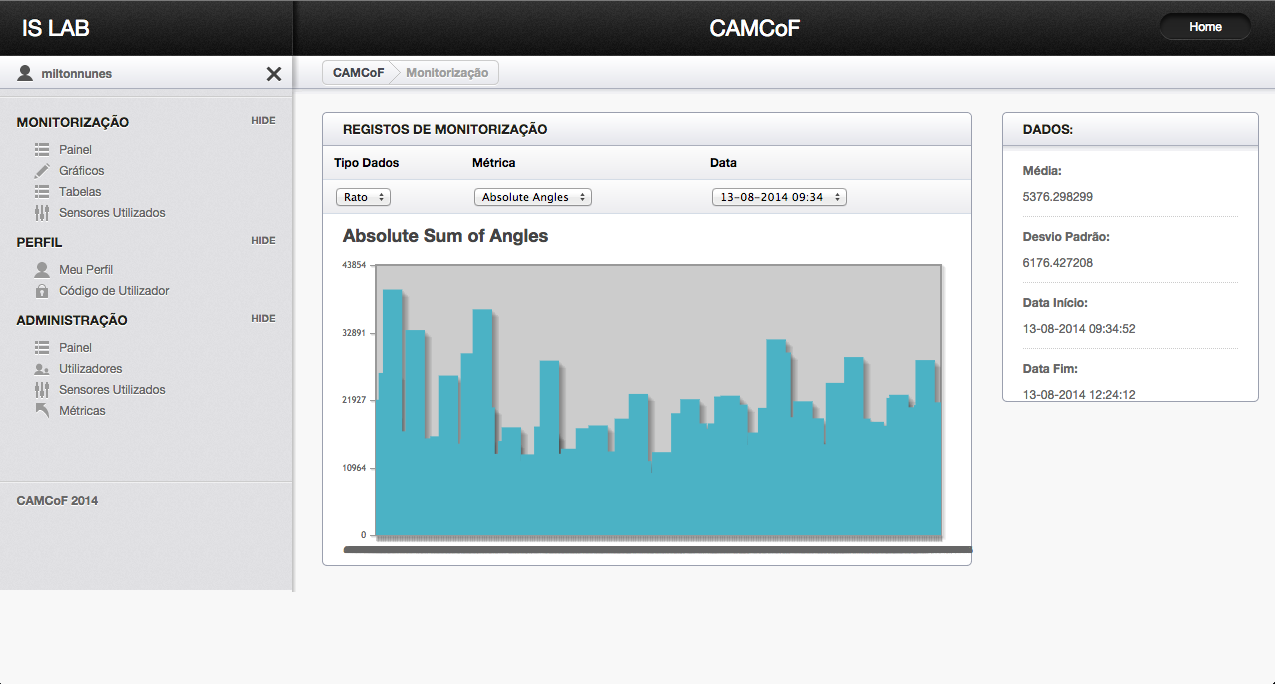
\includegraphics[scale=0.29]{Images/graphs.png}
   \caption{Página de visualização de registos de monitorização sob a forma de gráficos}
\end{figure}


\section{Funcionalidades de Administração}

Relativamente às funcionalidades de administração, estas residem sobretudo no acesso a informação privilegiada. Tem como principal objetivo acompanhar a utilização da arquitetura e poder aceder a informações relativas a essa utilização. Desta forma, para além dos dados estatísticos apresentados no painel de administração, no qual pode, por exemplo, saber que utilizadores estão a ser monitorizados e quais os sensores utilizados no momento, o administrador tem acesso a outros conteúdos relevantes.

\begin{figure}[htb]
   \centering
   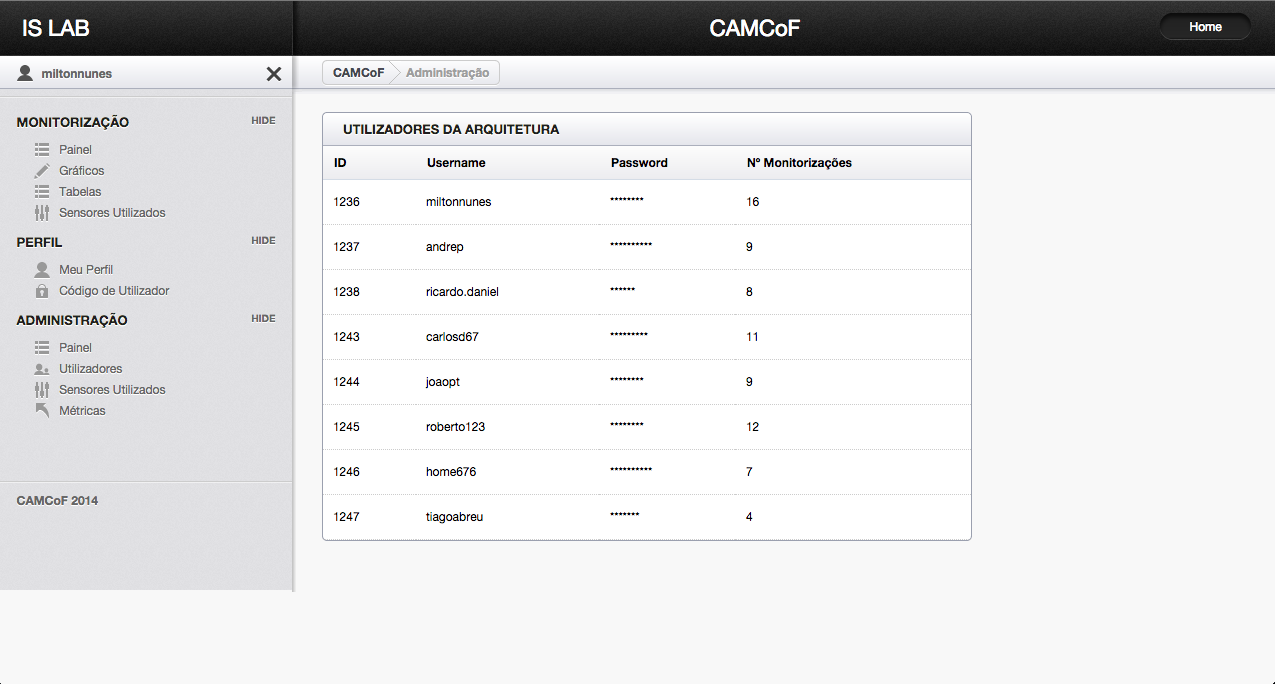
\includegraphics[scale=0.29]{Images/users.png}
   \caption{Página de consulta de utilizadores da arquitetura}
\end{figure}

Cada administrador do sistema poderá consultar os dados de todos os utilizadores do sistema, podendo ver não só os seus dados, como também saber o número de monitorizações efetuado por cada um. Para além das informações relativas a utilizadores da arquitetura, o administrador tem também acesso aos registos dos sensores utilizados na arquitetura, independentemente do momento da sua utilização e ainda à lista de todas as métricas integradas na arquitetura. Todo este conjunto de funcionalidades permite a cada administrador acompanhar a utilização da arquitetura e aceder aos seus dados principais.

\begin{figure}[htb]
   \centering
   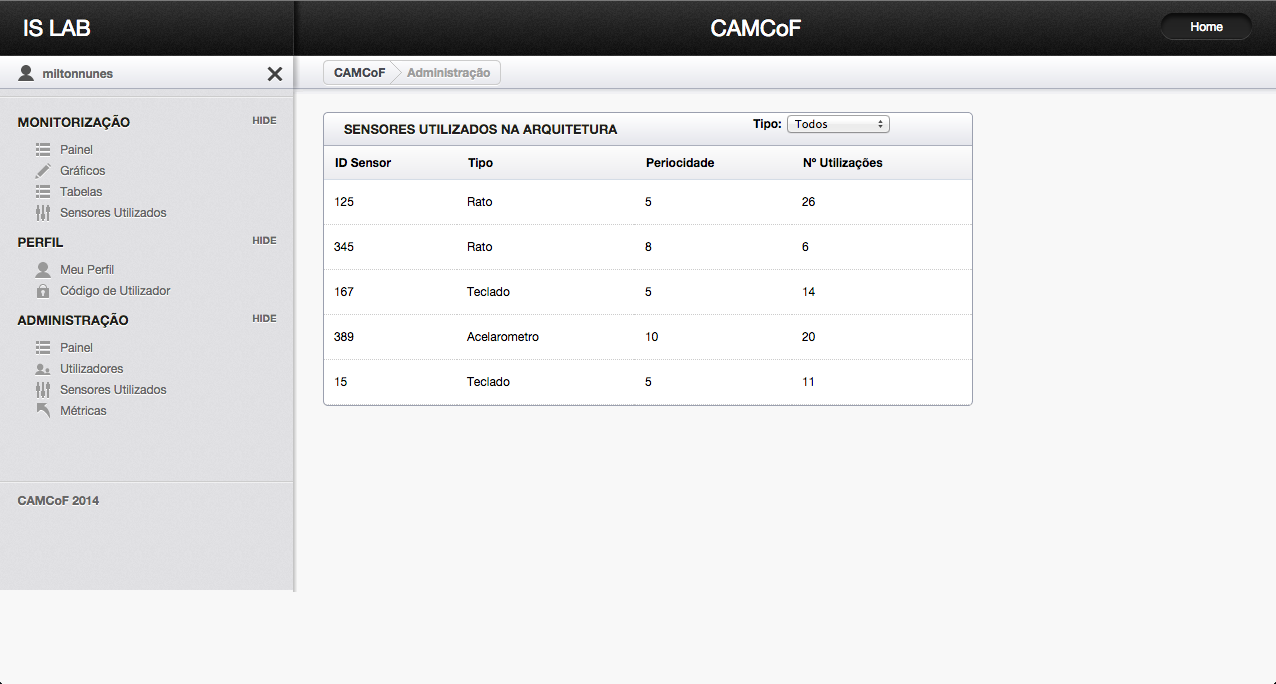
\includegraphics[scale=0.29]{Images/sensores.png}
   \caption{Página de consulta de sensores registados na arquitetura}
\end{figure}


\section{Conclusão}

O padrão MVC utilizado no desenvolvimento desta plataforma revelou-se bastante útil e contribuiu para que a implementação da interface fosse um processo mais rápido do que seria expectável. A separação de componentes da aplicação e tratamento de cada função em específico na respetiva camada contribui para a simplificação do desenvolvimento da interface e consequentemente tornou o processo mais rápido e intuitivo. Apesar de não se tratar de uma aplicação com elevada complexidade, o potencial e capacidade deste padrão ficou bem patente no processo de desenvolvimento e demonstrou o porquê da utilização massiva deste padrão atualmente.

Quanto à interface construída, esta será certamente de grande utilidade não só para os utilizadores da arquitetura, como também para os administradores da aplicação. O objetivo consistiu em abranger ao máximo a arquitetura e a sua informação, não só resultante da monitorização mas também toda a que está diretamente relacionada com isso e com o funcionamento da arquitetura. Objetivo esse que se pode afirmar ter sido alcançado, sendo possível aos seus utilizadores aceder aos dados mais relevantes da arquitetura, consoante o seu nível de acesso na interface.

No caso concreto da apresentação dos dados relativos à monitorização e estatísticas diretamente relacionadas, estas foram implementadas da forma idealizada. Os dados estatísticos presentes nas páginas principais de cada tipo de utilizador dão pequenas, mas importantes, informações sobre a utilização da arquitetura, tanto relativamente ao utilizador em questão como à utilização efetuada por todos os utilizadores. Quanto às formas de apresentação dos resultados de monitorização foram desenvolvidas com o intuito de permitir ao utilizador aceder de forma mais genérica e de fácil interpretação aos registos através dos gráficos. No caso do utilizador pretender um acesso e análise mais pormenorizada poderá fazê-lo através das tabelas de registos. Todas estas funcionalidades foram implementadas com o intuito de permitir um acesso simples e prático a este conjunto de dados fundamentais.

Deste modo pode-se concluir que a interface criada é um importante complemento à arquitetura e às suas funcionalidades e uma ferramenta extremamente útil para os seus utilizadores. Tendo por base uma arquitetura que permite a recolha de diferentes tipos de informação, de forma distribuída, e o seu tratamento e agregação, era importante a existência de uma ferramenta que permitisse a consulta dos dados resultantes. Através da interface desenvolvida os utilizadores da arquitetura podem assim consultar de forma simples e intuitiva o resultado das suas monitorizações e informação relacionada. Esta interface web permite também comprovar a funcionalidade da arquitetura e verificar a sua capacidade de recolha e gestão da informação.

 

\chapter{Conclusão}

 

\newpage
\thispagestyle{empty}
\mbox{}






%% ----------------------------------------------------------------
% Now begin the Appendices, including them as separate files

\addtocontents{toc}{\vspace{2em}} % Add a gap in the Contents, for aesthetics

\appendix % Cue to tell LaTeX that the following 'chapters' are Appendices

%% Appendix A

\chapter{Results Tables}
\addtotoc{Appendix A}
\label{Appendix}
\lhead{Appendix A. \emph{Results Tables}}







 	% Appendix Title


%\input{./Appendices/AppendixB} % Appendix Title

%\input{./Appendices/AppendixC} % Appendix Title

\addtocontents{toc}{\vspace{2em}}  % Add a gap in the Contents, for aesthetics
\backmatter

%% ----------------------------------------------------------------
%\pagebreak
%\bibliographystyle{plain}
%\bibliography{teseBibtex.bib}
%\pagebreak

\bibliographystyle{plain}  % Use the "unsrtnat" BibTeX style for formatting the Bibliography
\bibliography{teseBibtex}  % The references (bibliography) information are stored in the file named "Bibliography.bib"

\pagebreak





\end{document}  % The End


%% ----------------------------------------------------------------